\chapter{Substructural logical specifications}
\label{chapter-framework}

In this chapter, we design a logical framework of
substructural logical specifications (\sls). The framework is
justified as a fragment of the logic \ollll~from Chapter~3, though we
modify the presentation significantly, both to simplify the appearance
of proof terms and to facilitate writing down and manipulating partial
proofs.

The specifics of the domain of first-order quantification in
\ollll~were omitted in Chapter~3, so in
Section~\ref{sec:sls-termlanguage} we give a careful presentation of
the term language for \sls, Spine Form LF. 
%
In Section~\ref{sec:slsframework} we present \sls~as a fragment of
\ollll, and in Section~\ref{sec:framework-concurrenteq} we discuss
{\it concurrent equality}, a coarser equivalence on \sls~proof
terms than the one given by focused \ollll. 
%
In Section~\ref{sec:sls-adequate} we adopt the methodology of adequate
encoding from LF to \sls, in the process introducing {\it generative
  signatures}, which play a critical role in Part 3 of this thesis.
%
In Section~\ref{sec:prototype} we cover the \sls~prototype
implementation, and in Section~\ref{sec:framework-logicprog} we review
some intuitions about logic programming in the framework. 
%
Finally, in Section~\ref{sec:designdecisions}, we discuss some of the
decisions reflected in the design of \sls~and how some decisions could
have been potentially been made differently.

\section{Spine Form LF as a term language}
\label{sec:sls-termlanguage}

Other substructural logical frameworks, like Cervesato and Pfenning's
LLF \cite{cervesato02linear}, Polakow's OLF \cite{polakow01ordered},
and Watkins et al.'s CLF \cite{watkins02concurrent} are {\it
  fully-dependent type theories}: the language of terms (that is, the
domain of first-order quantification) is the same as the language of
proof terms, the representatives of logical derivations (we will call
the domain of quantification the {\it object terms} when ``terms''
would be ambiguous). The logical framework \sls~presented in this
chapter breaks from this tradition. The domain of first-order
quantification, which was left unspecified in Chapter 3, will be
presently described as Spine Form LF, a well-understood logical
framework derived from the normal forms of the purely persistent type
theory LF \cite{harper93framework}.

All the information in this section is standard and adapted from
various sources, especially Harper, Honsell, and Plotkin's original
presentation of LF \cite{harper93framework}, Cervesato and Pfenning's
discussion of spine form terms \cite{cervesato02linear}, Watkins et
al.'s presentation of the canonical forms of CLF
\cite{watkins02concurrent}, Nanevski et al.'s dependent contextual
modal type theory \cite{nanevski08contextual}, Harper and Licata's
discussion of Canonical LF \cite{harper07mechanizing}, and Reed's
spine form presentation of HLF \cite{reed09hybrid}.

It would be entirely consistent for us to appropriate Harper and
Licata's Canonical LF presentation instead of presenting Spine Form
LF. Nevertheless, a spine-form presentation of canonical LF serves to
make our presentation more uniform, as spines are used in the proof
term language of \sls. Canonical term languages like Canonical LF
correspond to normal natural deduction presentations of logic, whereas
spine form term languages correspond to focused sequent calculus
presentations like the ones we have considered thus far.

\subsection{Core syntax}

The syntax of Spine Form LF is extended in two places to handle \sls:
rules ${\sf r} : A^-$ in the signature contain negative \sls~types
$A^-$ (it would be possible to separate out the LF portion of
signatures from the \sls~rules), and several new base kinds
are introduced for the sake of \sls~-- ${\sf prop}$, ${\sf prop}\,{\sf
  ord}$, ${\sf prop}\,{\sf lin}$, and ${\sf prop}\,{\sf pers}$.
% We also add four additional kinds, ${\sf prop}$, which classifies
% negative ordered atomic types $p^-$, ${\sf prop}\,{\sf ord}$, which
% classifies positive ordered atomic types $p^+$, ${\sf prop}\,{\sf
%   lin}$, which classifies positive linear/mobile/ephemeral atomic
% types $p^+_\meph$, and ${\sf prop}\,{\sf ord}$, which classifies
% positive persistent atomic types $p^+_\mpers$.  Other than the extra
% kinds classifying atomic \sls~propositions, kinds $\kappa$ are
% otherwise exactly as they are in other presentations of LF; kinds
% classify types $\tau$, and types $\tau$ classify normal terms
% $\lf{t}$ and spines $\lf{\spi}$. Kinds $\kappa$ and types $\tau$ are
% both treated as syntactic refinements of {\it classifiers} $\nu$.
\begin{align*}
& \mbox{Signatures} & \Sigma & ::= \cdot 
  \mid \Sigma, \lf{\sf c} : \tau
  \mid \Sigma, {\sf a} : \kappa
  \mid \Sigma, {\sf r} : A^-
\\
& \mbox{Variables} & \lf{a}, \lf{b} & ::= \ldots
\\
& \mbox{Variable contexts} & \Psi & ::= \cdot
  \mid \Psi, \lf{a} {:} \tau 
\\
& \mbox{Classifiers} & \nu & ::= \lfpi{x}{\nu}{\nu'} \mid {\sf type}
  \mid {\sf prop}
  \mid {\sf prop}\,{\sf ord}
  \mid {\sf prop}\,{\sf lin}
  \mid {\sf prop}\,{\sf pers}
  \mid \lfroot{\sf a}{\spi}
\\
& \mbox{Heads} & \lf{h} & ::= \lf{a} \mid \lf{\sf c}
\\
& \mbox{Normal terms} & \lf{t}, \lf{s} & ::= \lf{\lambda a.t}
  \mid \lf{\lfroot{h}{\spi}}
\\
& \mbox{Spines} & \lf{\spi} & ::= \lf{t; \spi} \mid \lf{\lfnil}
\\
& \mbox{Substitutions} & \lf{\sigma} & ::= \lf{\cdot}
  \mid \lf{t/a, \sigma}
  \mid \lf{b/\!\!/a, \sigma}
\end{align*}
\noindent
There are three important refinements of the language of classifiers $\nu$:
\smallskip
\begin{itemize}
\item Types $\tau$ are either function types $\lfpi{a}{\tau}{\tau'}$
  or base types $\lfroot{\sf a}{\spi}$.
\item Kinds $\kappa$ are either families $\lfpi{a}{\tau}{\kappa}$ or
  one of the base kinds: ${\sf type}$, ${\sf prop}$, ${\sf prop}\,{\sf
    ord}$, ${\sf prop}\,{\sf lin}$, or ${\sf prop}\,{\sf pers}$.
\item Atomic classifiers $p$ have the form $\lfroot{\sf a}{\spi}$.
\end{itemize}
\smallskip

LF spines $\lf\spi$ are just sequences of terms $\lf{(t_1; (\ldots;
  (t_n;())\ldots))}$; we will follow common convention and write
$\lf{h\,t_1\ldots t_n}$ as a convenient shorthand for the atomic term
$\lf{\lfroot{h}{(t_1; \ldots; (t_n;())\ldots)}}$; similarly, we will
write ${\sf a}\,\lf{t_1\ldots t_n}$ as a shorthand for atomic
classifiers $\lfroot{\sf a}{(t_1;
  (\ldots; (t_n;())\ldots))}$. % This shorthand evokes a canonical-forms
% presentation, as an atomic term, type, or proposition is a head
% $\lf{h}$ or ${\sf a}$ with the terms $\lf{t_1\ldots t_n}$ applied to
% it.

\begin{figure}[t]
\begin{align*}
\fbox{$\subst{\lf{t}}{\lf{\spi}}$}
\\
\subst{(\lf{\lambda a. t'})}{(\lf{t; \spi})}
 & = \subst{\rsubst{\lf{t}}{\lf{a}}{\lf{t'}}}{\lf{\spi}}
\\
\subst{\lfroot{\lf h}{\spi}}{\lfnil}
 & = \lfroot{\lf h}{\spi}
\end{align*}\begin{align*}
\fbox{$\rsubst{\lf{t}}{\lf{a}}{\lf{\spi}}$}&
&
\fbox{$\rsubst{\lf{t}}{\lf{a}}{\lf{t'}}$}&
&
\\
\rsubst{\lf t}{\lf a}{(\lf{t'; \spi})}
 & = \lf{\no{\rsubst{\lf t}{\lf a}{\lf{t'}}}; 
         \no{\rsubst{\lf t}{\lf a}{\lf{\spi}}}} &
\rsubst{\lf t}{\lf a}(\lf{\lambda y. t'})
 & = \lf{\lambda b.\, \no{\rsubst{\lf t}{\lf a}{\lf{t'}}}} 
      & (\lf a \neq \lf b) 
\\
\rsubst{\lf t}{\lf a}{\lfnil} 
 & = \lfnil &
\rsubst{\lf t}{\lf a}{(\lf{\lfroot{a}{\spi}})}
 & = \subst{\lf t}{\rsubst{\lf t}{\lf a}{\lf{\spi}}}
\\
& & 
\rsubst{\lf t}{\lf a}{(\lf{\lfroot{h}{\spi}})}
 & = \lfroot{\lf h}{\no{\rsubst{\lf t}{\lf a}{\lf{\spi}}}}
      & ({\it if}~ \lf{h} \neq \lf{a})
\end{align*}
\caption{Hereditary substitution on terms, spines, and classifiers}
\label{fig:lf-hsubst}
\end{figure}

\subsection{Simple types and hereditary substitution}

In addition to LF types like $\lfpi{a}{(\lfpi{z}{(\lfroot{\sf
      a1}{\spi_1})}{\,(\lfroot{\sf
      a2}{\spi_2})})}{\,\lfpi{y}{(\lfroot{\sf
      a3}{\spi_3})}{\,(\lfroot{\sf a4}{\spi_4})}}$, both Canonical LF
and Spine Form LF take {\it simple types} into consideration. The
simple type corresponding to the type above is $({\sf a1} \supset {\sf
  a2}) \supset {\sf a3} \supset {\sf a4}$, where ${\supset}$
associates to the right. The simple type associated with
$\tau$ can is given by the function ${\mid}\tau{\mid}^- = \tau_s$, where
${\mid}\lfroot{\sf a}{\spi}{\mid}^- = {\sf a}$ and
${\mid}\lfpi{a}{\tau}{\tau'}{\mid}^- = {\mid}\tau{\mid}^- \supset
{\mid}\tau'{\mid}^-$. 


\begin{figure}
\begin{align*}
\fbox{$\lf{\sigma}(\lf{\spi})$}&
&
\fbox{$\lf{\sigma}(\lf{t'})$}
\\
\lf{\sigma}(\lf{t'; \spi}) 
 & = \lf{\no{\lf{\sigma}(\lf{t'})}; \no{\lf{\sigma}(\lf{\spi})}} &
\lf{\sigma}(\lf{\lambda a.t'}) 
 & = \lf{\lambda a.\,\no{\lf{(\sigma, a/\!\!/a)}(\lf{t'})}}
 & (\lf{a} \# \lf{\sigma})
\\
\lf{\sigma}\lfnil 
 & = \lfnil &
\lf{\sigma}(\lf{\lfroot{a}{\spi}}) 
 & = \subst{\lf t}{\no{\lf{\sigma}(\lf{\spi})}}
      & \lf{t/a} \in \lf{\sigma} 
\\
& &
\lf{\sigma}(\lf{\lfroot{a}{\spi}}) 
 & = \lf{\lfroot{b}{\no{\lf{\sigma}(\lf{\spi})}}} 
      & \lf{b/\!\!/a} \in \lf{\sigma} 
\\
& &
\lf{\sigma}(\lf{\lfroot{\sf c}{\spi}}) 
 & = \lf{\lfroot{\sf c}{\no{\lf{\sigma}(\lf{\spi})}}} 
\end{align*}\begin{align*}
\fbox{$\lf{\sigma}{\nu}$} &
\\
\lf{\sigma}(\lfpi{b}{\nu}{\nu'})
 & = \lfpi{b}{\lf{\sigma}\nu}{\,\lf{(\sigma, b/\!\!/b)}\nu'}
     \qquad (\lf a \neq \lf b) 
\\
\lf{\sigma}({\sf type})
  & = {\sf type}
\\ 
\lf{\sigma}({\sf prop}) 
 & = {\sf prop} 
\\
\lf{\sigma}({\sf prop}\,{\sf ord}) 
 & = {\sf prop}\,{\sf ord} 
\\
\lf{\sigma}({\sf prop}\,{\sf lin}) 
 & = {\sf prop}\,{\sf lin} 
\\
\lf{\sigma}({\sf prop}\,{\sf pers}) 
 & = {\sf prop}\,{\sf pers} 
\\
\lf{\sigma}(\lfroot{\sf a}{\spi}) 
 & = \lfroot{\sf a}{{\lf{\sigma\spi}}}
\end{align*}
\caption{Simultaneous substitution on terms, spines, and classifiers}
\label{fig:simsubst}
\end{figure}

Variables and constants are treated as having an intrinsic simple
type; these intrinsic simple types are sometimes written explicitly as
annotations $\lf{a}^{\tau_s}$ or $\lf{\sf c}^{\tau_s}$ (see
\cite{pfenning08church} for an example), but we will leave them
implicit.  An atomic term $\lf{h\,t_1\ldots t_n}$ must have an an
simple atomic type ${\sf a}$. This means that the head $\lf h$ must
have simple type $\tau_{s1} \supset \ldots \supset \tau_{sn} \supset
{\sf a}$ and each $\lf{t_i}$ much have simple type
$\tau_{si}$. Similarly, a lambda term $\lf{\lambda a. t}$ must have
simple type $\tau_s \supset \tau_s'$ where $\lf a$ is a variable with
simple type $\tau_s$ and $\lf t$ has simple type $\tau_s'$.

Simple types, which are treated with more care elsewhere
\cite{harper07mechanizing,reed09hybrid}, are critical because they
allow us to define hereditary substitution and hereditary reduction as
total functions in Figure~\ref{fig:lf-hsubst}. Intrinsically-typed
Spine Form LF terms correspond to the proof terms for a focused
presentation of (non-dependent) minimal logic. Hereditary reduction
$\subst{\lf{t}}{\lf{\spi}}$ and hereditary substitution $\rsubst{\lf
  t}{\lf a}{\lf{t'}}$, which are both implicitly indexed by the simple
type $\tau_s$ of $\lf t$, capture the computational content of
structural cut admissibility on these proof terms.

\subsection{Judgments}

Hereditary substitution is necessary to define simultaneous
substitution into types and terms in Figure~\ref{fig:simsubst}.  We
will treat simultaneous substitutions in a mostly informal way,
relying on the more careful treatment by Nanevski et
al.~\cite{nanevski08contextual}. In particular, we write $\lf{[t/a]}$
for a simultaneous substitution that acts as the identity on all
variables except for $\lf{a}$; this notation is used in the definition
of LF typing in in Figure~\ref{fig:lf-form}, which is adapted to Spine
Form LF from Harper and Licata's Canonical LF presentation
\cite{harper07mechanizing}. The judgments $\lf{a}\#\lf{\sigma}$,
$\lf{a}\#\Psi$, $\lf{\sf c}\#\Sigma$, ${\sf a}\#\Sigma$, and ${\sf
  r}\#\Sigma$ assert that the relevant variable or constant does not
already appear in the context $\Psi$ (as a binding $\lf{a}{:}\tau$),
the signature $\Sigma$ (as a declaration $\lf{\sf c} : \tau$, ${\sf a}
: \nu$, or ${\sf r} : A^-$), or the substitution $\lf{\sigma}$ (as a
binding $\lf{t/a}$ or \mbox{$\lf{b/\!\!/a}$}).

\begin{figure}
\fbox{$\vdash_\subord \Sigma\,{\sf sig}$}\vspace{-10pt}
\[
\infer
{\vdash_\subord \cdot\,{\sf sig} \mathstrut}
{}
\quad
\infer
{\vdash_\subord (\Sigma, \lf{\sf c} : \tau)\,{\sf sig} \mathstrut}
{\vdash_\subord \Sigma\,{\sf sig} 
 &
 \cdot \vdash_{\Sigma,\subord} \tau\,{\sf type}
 &
 \tau \prec_\subord \tau
 &
 \lf{\sf c} \# \Sigma \mathstrut}
\]
\[
\infer
{\vdash_\subord (\Sigma, {\sf a} : \kappa)\,{\sf sig} \mathstrut}
{\vdash_\subord \Sigma\,{\sf sig}
 &
 \vdash_{\Sigma, \subord} \kappa \,{\sf kind}
 &
 \kappa  \sqsubset_\subord {\sf a} 
 &
 {\sf a} \# \Sigma\mathstrut}
\quad
\infer
{\vdash_\subord (\Sigma, {\sf r} : A^-)\,{\sf sig} \mathstrut}
{\vdash_\subord \Sigma\,{\sf sig}
 &
 \vdash_{\Sigma, \subord} A^- \,{\sf prop}^-
 &
 {\sf r} \# \Sigma \mathstrut}
\]

\medskip
\fbox{$\vdash_{\Sigma,\subord} \Psi\,{\sf ctx}$} -- presumes
  $\vdash_{\subord} \Sigma\,{\sf sig}$\vspace{-10pt}
\[
\infer
{\vdash_{\Sigma,\subord} \cdot\,{\sf ctx} \mathstrut}
{}
\quad
\infer
{\vdash_{\Sigma,\subord} (\Psi, \lf{a}{:}\tau)\,{\sf ctx} \mathstrut}
{\vdash_{\Sigma,\subord} \Psi\,{\sf ctx}
 &
 \Psi \vdash_{\Sigma, \subord} \tau\,{\sf type}
 &
 \lf a \# \Psi}
\]

\medskip
\fbox{$\Psi \vdash_{\Sigma,\subord} \kappa\,{\sf kind}$} -- presumes
  $\vdash_{\Sigma, \subord} \Psi\,{\sf ctx}$
\[
\infer
{\Psi \vdash_{\Sigma,\subord} (\lfpi{a}{\tau}{\kappa})\,{\sf kind} \mathstrut}
{\Psi \vdash_{\Sigma,\subord} \tau\,{\sf type}
 &
 \Psi, \lf{a}{:}\tau \vdash_{\Sigma,\subord} \kappa\,{\sf kind}}
\quad
\infer{\Psi \vdash_{\Sigma,\subord} {\sf type}\,{\sf kind} \mathstrut}{}
\quad
\infer{\Psi \vdash_{\Sigma,\subord} {\sf prop}\,{\sf kind} \mathstrut}{}
\]
\[
\infer
{\Psi \vdash_{\Sigma,\subord} ({\sf prop}\,{\sf ord})\,{\sf kind}\mathstrut}{}
\quad
\infer
{\Psi \vdash_{\Sigma,\subord} ({\sf prop}\,{\sf lin})\,{\sf kind}\mathstrut}{}
\quad
\infer
{\Psi \vdash_{\Sigma,\subord} ({\sf prop}\,{\sf pers})\,{\sf kind}\mathstrut}{}
\]

\medskip
\fbox{$\Psi \vdash_{\Sigma,\subord} \tau\,{\sf type}$} -- presumes
  $\vdash_{\Sigma, \subord} \Psi\,{\sf ctx}$
\[
\infer
{\Psi \vdash_{\Sigma,\subord}(\lfpi{a}{\tau}{\tau'})\,{\sf type} \mathstrut}
{\Psi \vdash_{\Sigma,\subord} \tau\,{\sf type}
 &
 \Psi, \lf{a}{:}\tau \vdash_{\Sigma,\subord} \tau'\,{\sf type}
 &
 \tau \preceq_\subord \tau' \mathstrut}
\quad
\infer
{\Psi \vdash_{\Sigma,\subord}(\lfroot{\sf a}{\spi})\,{\sf type} \mathstrut}
{a{:}\kappa \in \Sigma
 &
 \Psi, [\kappa] \vdash_{\Sigma,\subord} \lf{\spi} : {\sf type}
 \mathstrut}
\]

\medskip
\fbox{$\Psi \vdash_{\Sigma,\subord} t : \tau$} -- presumes 
  $\Psi \vdash_{\Sigma,\subord} \tau\,{\sf type}$
\[
\infer
{\Psi \vdash_{\Sigma,\subord} \lf{\lambda a.t} : \lfpi{x}{\tau}{\tau'}\mathstrut}
{\Psi, \lf{a}{:}\tau \vdash_{\Sigma,\subord} \lf{t} : \tau'\mathstrut}
\quad
\infer
{\Psi \vdash_{\Sigma,\subord} \lf{\lfroot{\sf c}{\spi}} : p
 \mathstrut}
{\lf{\sf c} : \tau \in {\Sigma}
 &
 \Psi, [\tau] \vdash_{\Sigma,\subord} \lf{\spi} : \tau'
 &
 \tau' = p\mathstrut}
\]
\[
\infer
{\Psi \vdash_{\Sigma,\subord} \lf{\lfroot{a}{\spi}} : p
 \mathstrut}
{\lf{a} {:} \tau \in {\Psi}
 &
 \Psi, [\tau] \vdash_{\Sigma,\subord} \lf{\spi} : \tau'
 &
 \tau' = p}
\]

\medskip
\fbox{$\Psi, [\nu] \vdash_{\Sigma,\subord} \lf{\spi} : \nu_0$} --
presumes that either $\Psi \vdash_{\Sigma,\subord} \nu\, {\sf type}$
or that $\Psi \vdash_{\Sigma,\subord} \nu\, {\sf kind}$
\[
\infer
{\Psi, [\nu] \vdash_{\Sigma,\subord} \lfnil : \nu \mathstrut}
{}
\quad
\infer
{\Psi, [\lfpi{a}{\tau}{\nu}] \vdash_{\Sigma,\subord} \lf{t; \spi} : \nu_0
 \mathstrut}
{\Psi \vdash_{\Sigma,\subord} \lf{t} : \tau
 &
 \lf{[t/a]}\nu = \nu'
 &
 \Psi, [\nu'] \vdash_{\Sigma,\subord} \lf{\spi} : \nu_0 \mathstrut}
\]

\medskip
\fbox{$\Psi \vdash \lf{\sigma} : \Psi'$} -- presumes
 $\vdash_{\Sigma,\subord} \Psi\,{\sf ctx}$
 and
 $\vdash_{\Sigma,\subord} \Psi'\,{\sf ctx}$
\[
\infer
{\Psi \vdash_{\Sigma,\subord} \cdot : \cdot \mathstrut}
{}
\quad
\infer
{\Psi \vdash_{\Sigma,\subord} (\lf{\sigma, t/a}) : \Psi', \lf{a}{:}\tau
  \mathstrut}
{\Psi \vdash_{\Sigma,\subord} \lf{\sigma} : \Psi' 
 &
 \Psi \vdash_{\Sigma,\subord} \lf{t} : \lf{\sigma}\tau 
  \mathstrut}
\quad
\infer
{\Psi \vdash_{\Sigma,\subord} (\lf{\sigma, b/\!\!/a}) : \Psi', \lf{a}{:}\tau
  \mathstrut}
{\Psi \vdash_{\Sigma,\subord} \lf{\sigma} : \Psi'
 &
 \lf{b}{:}\lf{\sigma}\tau \in \Psi
  \mathstrut}
\]

\caption{LF formation judgments.}
\label{fig:lf-form}
\end{figure}

All the judgments in Figure~\ref{fig:lf-form} are indexed by a
transitive {\it subordination relation} $\subord$, similar to the one
introduced by Virga in \cite{virga99higherorder}. We treat $\subord$
as a binary relation on type family constants.  Let ${\sf head}(\tau)
= {\sf a}$ if $\tau =
\lfpi{a_1}{\tau_{1}}{\,.\,.\lfpi{a_{m}}{\tau_{m}}{\,\lfroot{\sf
      a}{\spi}}}$. The signature formation operations depend on three
judgments. The index subordination judgment, $\kappa \sqsubset_\subord
{\sf a}$, relates type family constants to types. 
%
It is always the case that $\kappa =
\lfpi{a_1}{\tau_1}{\ldots\lfpi{a_n}{\tau_n}{\sf type}}$, and the
judgment $\kappa \sqsubset_\subord {\sf a}$ holds if $({\sf
  head}(\tau_i), {\sf a}) \in \subord$ for $1 \leq i \leq n$.
%
The type subordination judgment $\tau \prec_\subord \tau'$ holds if
$({\sf head}(\tau), {\sf head}(\tau')) \in \subord$, and the judgment
$\tau \preceq_\subord \tau'$ is the symmetric extension of this
relation.

There are a number of well-formedness theorems that we need to
consider, such as the fact that substitutions compose in a
well-behaved way and that hereditary substitution is always
well-typed.  However, as these theorems are adequately covered
elsewhere, we will proceed with using LF as a term language and will 
treat term-level operations like substitution somewhat informally.

While we will include the annotations for signature $\Sigma$
and the subordination relation $\subord$ in the definitions of section
and the next one, in the future we will often leave the signature
$\Sigma$ implicit when it is unambiguous or unimportant. We will
almost always leave the subordination relation implicit; we can assume
where applicable that we are working with the {\it strongest} (that
is, the smallest) subordination relation of the given signature
\cite{harper07mechanizing}.

\subsection{Adequacy}
\label{sec:lf-adequacy}

{\it Adequacy} was the name given by Harper, Honsell, and Plotkin to
the methodology of connecting inductive definitions to the canonical
forms of a particular type family in LF. Consider, as a standard
example, the untyped lambda calculus, which is generally specified by
a BNF grammar such as the following:
\[
\obj{e} ::= \obj{x} \mid \obj{\lambda x.e} \mid \obj{e_1\,e_2}
\]
We can adequately encode this language of terms into LF (with a
subordination relation $\subord$ such that $({\sf exp}, {\sf
  exp}) \in \subord$) by giving the following signature:
\begin{align*}
\Sigma & = \cdot, 
\\
 & ~\quad {\sf exp} : {\sf type}, 
\\
 & ~\quad \lf{\sf app} : 
     \lfpi{a}{{\sf exp}}{\,\lfpi{b}{\sf exp}{\,\sf exp}},
\\
 & ~\quad \lf{\sf lam} : 
     \lfpi{a}{(\lfpi{b}{\sf exp}{\,\sf exp})}{\,\sf exp}
\end{align*}
Note that the variables $\lf{a}$ and $\lf{b}$ are bound by
$\Pi$-quantifiers in the declaration of $\lf{\sf app}$ and $\lf{\sf lam}$ but
never used. The usual convention is to abbreviate
$\lfpi{a}{\tau}{\tau'}$ as $\tau \rightarrow \tau'$ when $\lf{a}$ is
not free in $\tau'$, which would give $\lf{\sf app}$ type ${\sf exp}
\rightarrow {\sf exp} \rightarrow {\sf exp}$ and $\lf{\sf lam}$ type
$({\sf exp} \rightarrow {\sf exp}) \rightarrow {\sf exp}$.

\bigskip
\begin{theorem}[Adequacy for terms]\label{thm:expadequacy}
  Up to standard $\alpha$-equivalence, there is a bijection between
  expressions $\obj{e}$ (with free variables in the set
  $\{\obj{x_1},\ldots,\obj{x_n}\}$) and Spine Form LF terms $\lf{t}$ such
  that $\lf{x_1}{:}\mathsf{exp}, \ldots, \lf{x_n}{:}\mathsf{exp} \vdash
  \lf{t} : \mathsf{exp}$. 
\end{theorem}

\begin{proof}
By induction on the structure of the inductive definition of $\obj{e}$
in the forward direction and by induction on the structure of 
terms $\lf{t}$ with type ${\sf exp}$ in the reverse direction.
\end{proof}

We express the constructive content of this theorem as a bijective
function $\interp{e} = \lf{t}$ from object language terms $\obj{e}$ to
representations LF terms $\lf{t}$ of type ${\sf exp}$. If we had also
defined substitution $\obj{[e/x]e'}$ on terms, it would be necessary
to show that the bijection is compositional: that is, that
$[\interp{e}/\lf{x}]\interp{e'} = \interp{[e/x]e'}$.  Note that
adequacy critically depends on the context having the form
$\lf{x_1}{:}{\sf exp},\ldots,\lf{x_n}{:}{\sf exp}$. If we had a
context with a variable $\lf{y}{:}({\sf exp} \rightarrow {\sf exp})$,
then we could form a term $\lf{y\,({\sf lam}\,\lambda x. x)}$ with
type ${\sf exp}$ that does {\it not} adequately encode any term
$\obj{e}$ in the untyped lambda calculus.

One of the reasons subordination is important in practice is that it
allows us to consider the adequate encoding of expressions in contexts
$\Psi$ that have other variables $\lf{x}{:}\tau$ as long as $({\sf
  head}(\tau),{\sf exp}) \notin \subord$. If $\Psi,\lf{x}{:}\tau
\vdash_{\Sigma,\subord} \lf{t} : {\sf exp}$ and $\tau
\not\preceq_\subord {\sf exp}$, then $\lf{x}$ cannot be free in
$\lf{t}$, so $\Psi \vdash_{\Sigma,\subord} \lf{t} : {\sf exp}$ holds as
well. By iterating this procedure, it may be possible to strengthen a
context $\Psi$ into one of the form $\lf{x_1}{:}{\sf
  exp},\ldots,\lf{x_n}{:}{\sf exp}$, in which case we can conclude
that $\lf t = \interp{e}$ for some untyped lambda calculus term $\obj
e$.



\section{The logical framework \sls}
\label{sec:slsframework}

In this section, we will describe a restricted set of polarized
\ollll~propositions and focused \ollll~proof terms that make up the
logical framework \sls. For the remainder of the thesis, we will work
exclusively with the following positive and negative
\sls~propositions, which are a syntactic refinement of the positive
and negative propositions of polarized \ollll:
\begin{align*}
A^+, B^+, C^+ & ::= p^+ \mid p^+_\meph \mid p^+_\mpers \mid {\downarrow}A^-
  \mid {\gnab}A^- \mid {!}A^- \mid \one \mid A^+ \fuse B^+
  \mid \exists \lf{a}{:}\tau.A^+ \mid \lf{t} \doteq_\tau \lf{s}
\\
A^-, B^-, C^- & ::= p^- \mid {\ocircle}A^+ \mid A^+ \lefti B^- 
  \mid A^+ \righti B^- \mid A^- \with B^-
  \mid \forall \lf{a}{:}\tau.A^-
\end{align*}
%Aside from the type annotation $\tau$ on unification $\lf{t}
%\doteq_\tau \lf{s}$ and on the quantifiers $\forall \lf{x}{:}\tau. A^-$
%and $\exists \lf{x}{:}\tau. A^+$, which we will in general leave implicit,
%this is exactly a refinement of the  
%Notably missing from this refinement are
%upshifts ${\uparrow}A^+$ and right-permeable atomic propositions
%$p^-_\mlax$.
% We will also continue to
% avoid using variable names $x$ with inverting positive propostiions
% and focused negative propositions. In the case of focused
% propositions, there is a straightforward justification: the form of
% context ensures there is at most one of them. In the case of positive
% propositions, we are justified by the convention discussed in the last
% chapter that we only ever frame off the leftmost positive proposition
% in the context.
We now have to deal with a point of notational dissonance: all
existing work on CLF, all existing implementations of CLF, and the
prototype implementation of \sls~(Section~\ref{sec:prototype}) use the
notation $\{ A^+ \}$ for the connective internalizing the judgment
$\islax{A^+}$, which we have written as ${\ocircle}A^+$, following
Fairtlough and Mendler \cite{fairtlough95propositional}. The
traditional notation overloads curly braces, which we also use for
the context-framing notation 
$\tackon{\Theta}{\Delta}$ introduced in Section~\ref{sec:contexts}. We
will treat ${\ocircle}A^+$ and $\{ A^+ \}$ as synonyms in \sls, preferring the
former in this chapter and the latter afterwards.

Positive ordered atomic propositions
$p^+$ are atomic classifiers ${\sf a}\,\lf{t_1}\ldots\lf{t_n}$ with
kind ${\sf prop}\,{\sf ord}$, positive linear atomic propositions
$p^+_\meph$ and $p^+_\mpers$ are (respectively) atomic classifiers
with kind ${\sf prop}\,{\sf lin}$ and ${\sf prop}\,{\sf pers}$, and
negative ordered atomic propositions $p^-$ are atomic classifiers
with kind ${\sf prop}$.  From this point on,
we will unambiguously refer to atomic propositions $p^-$ as negative
atomic propositions, omitting ``ordered.'' Similarly, we will refer to
atomic propositions $p^+$, $p^+_\meph$, and $p^+_\mpers$ collectively
as positive atomic propositions but individually as ordered, linear,
and persistent propositions, respectively, omitting ``positive.''
(``Mobile'' and ``ephemeral'' will continue to be used as synonyms for
``linear.'')

\begin{figure}
\fbox{$\Psi; \mathcal S \vdash_{\Sigma,\subord} A^+\,{\sf prop}^+$} -- presumes
  $\vdash_{\Sigma,\subord} \Psi\,{\sf ctx}$ and $\mathcal S \subseteq \Psi$
\[
\infer
{\Psi; \mathcal S
   \vdash_{\Sigma,\subord} \lfroot{\sf a}{\spi}\,{\sf prop}^+ \mathstrut}
{{\sf a}{:}\kappa \in \Sigma
 &
 \Psi, [\kappa] \vdash_{\Sigma,\subord} \lf{\spi} : {\sf prop}\,{\sf ord} \mathstrut}
\quad
\infer
{\Psi; \mathcal S
   \vdash_{\Sigma,\subord} \lfroot{\sf a}{\spi}\,{\sf prop}^+ \mathstrut}
{{\sf a}{:}\kappa \in \Sigma
 &
 \Psi, [\kappa] \vdash_{\Sigma,\subord} \lf{\spi} : {\sf prop}\,{\sf lin} \mathstrut}
\]
\[
\infer
{\Psi; \mathcal S
   \vdash_{\Sigma,\subord} \lfroot{\sf a}{\spi}\,{\sf prop}^+ \mathstrut}
{{\sf a}{:}\kappa \in \Sigma
 &
 \Psi, [\kappa] \vdash_{\Sigma,\subord} \lf{\spi} : {\sf prop}\,{\sf pers} \mathstrut}
\]
\[
\infer
{\Psi; \mathcal S \vdash_{\Sigma,\subord} {\downarrow}A^-\,{\sf prop}^+ \mathstrut}
{\Psi; \cdot \vdash_{\Sigma,\subord} A^-\,{\sf prop}^- \mathstrut}
\quad
\infer
{\Psi; \mathcal S \vdash_{\Sigma,\subord} {\gnab}A^-\,{\sf prop}^+ \mathstrut}
{\Psi; \cdot \vdash_{\Sigma,\subord} A^-\,{\sf prop}^- \mathstrut}
\quad
\infer
{\Psi; \mathcal S \vdash_{\Sigma,\subord} {!}A^-\,{\sf prop}^+ \mathstrut}
{\Psi; \cdot \vdash_{\Sigma,\subord} A^-\,{\sf prop}^- \mathstrut}
\quad
\infer
{\Psi; \mathcal S \vdash_{\Sigma,\subord} \one\,{\sf prop}^+ \mathstrut}
{}
\] 
\[
\infer
{\Psi; \mathcal S_1, \mathcal S_2 \vdash_{\Sigma,\subord} A^+ \fuse B^+\,{\sf prop}^+ \mathstrut}
{\Psi; \mathcal S_1 \vdash_{\Sigma,\subord} A^+\,{\sf prop}^+ 
 &
 \Psi; \mathcal S_2 \vdash_{\Sigma,\subord} B^+\,{\sf prop}^+  \mathstrut}
\quad
\infer
{\Psi; \mathcal S \vdash_{\Sigma,\subord} \exists \lf{a}{:}\tau. A^+\,{\sf prop}^+ \mathstrut}
{\Psi \vdash_{\Sigma,\subord} \tau\,{\sf type}
 &
 \Psi, \lf{a}{:}\tau; \mathcal S, \lf{a}{:}\tau \vdash_{\Sigma,\subord} A^+\,{\sf prop}^+ \mathstrut}
\] 
\[
\infer
{\Psi; \mathcal S \vdash_{\Sigma,\subord} \lf{t} \doteq_p \lf{s}\,{\sf prop}^+}
{\Psi \vdash_{\Sigma,\subord} p\,{\sf type}
 &
 \Psi \vdash_{\Sigma,\subord} \lf{t} : p
 &
 \Psi \vdash_{\Sigma,\subord} \lf{s} : p
 & 
 p \not\prec_\subord p}
\]
\[
\infer
{\Psi; \mathcal S \vdash_{\Sigma,\subord} \lf{a} \doteq_p \lf{s}\,{\sf prop}^+}
{\Psi \vdash_{\Sigma,\subord} p\,{\sf type}
 &
 \Psi \vdash_{\Sigma,\subord} \lf{a} : p
 &
 \Psi \vdash_{\Sigma,\subord} \lf{s} : p
 & 
 \lf{a}{:}p \in \mathcal S}
\]


\medskip
\fbox{$\Psi \vdash_{\Sigma,\subord} A^-\,{\sf prop}^-$} -- presumes
  $\vdash_{\Sigma,\subord} \Psi\,{\sf ctx}$ and
  $\mathcal S \subseteq \Psi$
\[
\infer
{\Psi; \mathcal S
   \vdash_{\Sigma,\subord} \lfroot{\sf a}{\spi}\,{\sf prop}^- \mathstrut}
{{\sf a}{:}\kappa \in \Sigma
 &
 \Psi, [\kappa] \vdash_{\Sigma,\subord} \lf{\spi} : {\sf prop} \mathstrut}
\quad
\infer
{\Psi; \mathcal S \vdash_{\Sigma,\subord} {\ocircle}A^+\,{\sf prop}^- \mathstrut}
{\Psi; \cdot \vdash_{\Sigma,\subord} A^+ : {\sf prop}^+ \mathstrut}
\]
\[
\infer
{\Psi; \mathcal S_1, \mathcal S_2 \vdash_{\Sigma,\subord} A^+ \lefti B^-\,{\sf prop}^- \mathstrut}
{\Psi; \mathcal S_1 \vdash_{\Sigma,\subord} A^+\,{\sf prop}^+ 
 &
 \Psi; \mathcal S_2 \vdash_{\Sigma,\subord} B^-\,{\sf prop}^-  \mathstrut}
\quad
\infer
{\Psi; \mathcal S_1, \mathcal S_2 \vdash_{\Sigma,\subord} A^+ \righti B^-\,{\sf prop}^- \mathstrut}
{\Psi; \mathcal S_1 \vdash_{\Sigma,\subord} A^+\,{\sf prop}^+ 
 &
 \Psi; \mathcal S_2 \vdash_{\Sigma,\subord} B^-\,{\sf prop}^-  \mathstrut}
\] 
\[
\infer
{\Psi; \mathcal S \vdash_{\Sigma,\subord} A^- \with B^-\,{\sf prop}^- \mathstrut}
{\Psi; \mathcal S \vdash_{\Sigma,\subord} A^-\,{\sf prop}^- 
 &
 \Psi; \mathcal S \vdash_{\Sigma,\subord} B^-\,{\sf prop}^-  \mathstrut}
\quad
\infer
{\Psi; \mathcal S \vdash_{\Sigma,\subord} \forall \lf{a}{:}\tau. A^-\,{\sf prop}^- \mathstrut}
{\Psi; \mathcal S \vdash_{\Sigma,\subord} \tau\,{\sf type}
 &
 \Psi, \lf{a}{:}\tau; \mathcal S, \lf{a}{:}\tau \vdash_{\Sigma,\subord} A^-\,{\sf prop}^- \mathstrut}
\] 
\caption{\sls~proposition formation judgments}
\label{fig:sls-propform}
\end{figure}

The formation judgments for \sls~types are given in
Figure~\ref{fig:sls-propform}. Much of the complexity of the
presentation is needed to make sure that whenever we decompose a
positive proposition $\lf{s} \doteq \lf{t}$ we have that $\lf{s} =
\lf{a}$ for some variable $\lf{a}$ in the context. When this is the
case, $\lf{[t/a]}$, is always a most general unifier of $\lf{s} =
\lf{a}$ and $\lf{t}$, which in turn means that the higher-order
unification rule from \ollll
\[
\infer[{\doteq}_L]
{\foc{\Psi}{\frameoff{\Theta}{\lf{t} \doteq \lf{s}}}{U}}
{\forall(\Psi' \vdash \lf{\sigma} : \Psi).
 &
 \lf{\sigma t} = \lf{\sigma s}
 &
 \longrightarrow
 &
 \foc{\Psi'}{\tackon{\lf{\sigma}\Theta}{\cdot}}{\lf{\sigma} U}
 }
\]
is equivalent to a much simpler rule:
\[
\infer[{\doteq}_{\it yes}]
{\foc{\Psi, \lf{a}{:}\tau, \Psi'}{\frameoff{\Theta}{\lf{a} \doteq \lf{t}}}{U}}
{\foc{\Psi, \lf{[t/a]}\Psi'}{\tackon{\lf{[t/a]}\Theta}{\cdot}}{\lf{[t/a]} U}}
\]

There are two distinct conditions under which we can be sure that
unification problems always have a most general solution.  \smallskip
\begin{enumerate}
\item Equality at an atomic type $p$ that is {\it not subordinate
    to itself} ($p \not\prec_\subord p$) is always allowed.  This is
  reflected in the first formation rule for $\lf{t} \doteq
  \lf{s}$ in Figure~\ref{fig:sls-propform}. 

  Types that are not self-subordinate can only be inhabited by
  variables: that is, if $p \not\prec_\subord p$ and $\Psi
  \vdash_{\Sigma,\subord} \lf{t} : p$, then $\lf{t} = \lf{{a}}$ where
  $\lf{a}:p \in \Psi$. For any unification problem $\lf{{a}}
  \doteq \lf{{b}}$, both $\lf{[{a}/b]}$ and $\lf{[{b}/a]}$ are most
  general unifiers.

\item The second condition under which equality is allowed is when it
  is used as a {\it notational definition}
  \cite{pfenning99algorithms}. The subset $\mathcal S$ of the LF
  context is treated as an a multiset. The result of this treatment is
  that each variable bound by an existential quantifier $\exists
  \lf{a}{:}p.\,A^+$ or a universal quantifier $\forall
  \lf{a}{:}p.\,A^-$ can be associated with at most one proposition
  $\lf{a} \doteq \lf{t}$, where $\lf{t}$ is arbitrary. This condition
  is handled by the second formation rule for $\lf{t} \doteq \lf{s}$
  in Figure~\ref{fig:sls-propform}. The
  rule ${\ocircle}(\exists \lf{a}.\, \lf{a} \doteq \lf{t} \fuse
  \lf{a} \doteq \lf{s})$ does not satisfy this condition because the
  introduced variable $\lf{a}$ is associated with the left-hand side
  of two different equalities, $\lf{a} \doteq \lf{t}$ and $\lf{a}
  \doteq \lf{s}$, that together encode an arbitrary unification
  problem $\lf{t} \doteq \lf{s}$.


  The proposition $\lf{a} \doteq \lf{t}$ must be reachable from its
  associated quantifier without crossing a shift or an exponential --
  in Andreoli's terms, it must be in the same {\it monopole}
  (Section~\ref{sec:linsynthetic}).
  This is enforced by the formation rules for shifts and exponentials,
  which clear the subset $\mathcal S$ in their premise.  The
  proposition $\forall \lf{a}.\, {\downarrow}({\sf
    p}\,\lf{a}) \lefti \lf{a} \doteq \lf{t} \lefti {\sf p}\,\lf{t}$
  satisfies this condition but $\forall \lf{a}.\,\forall
  \lf{b}.\,{\ocircle}(\lf{a} \doteq \lf{b})$ does not ($\ocircle$
  breaks focus), and the proposition ${\ocircle}(\exists
  \lf{a}. \lf{a} \doteq \lf{t})$ satisfies this condition but
  ${\ocircle}(\exists \lf{a}.  {\uparrow}(\lf{a} \doteq \lf{t} \lefti
  {\sf p}\,\lf{a}))$ does not (${\uparrow}$ breaks focus).  

%   This restriction ensures that, if the unification appears on the
%   left, the left-hand side of the unification will always be a
%   variable $\lf{a}$, meaning that $\lf{[t/a]}$ is always a most
%   general unifier.  This usage of unification is essentially just a
%   notational definition \cite{pfenning99algorithms}.
\end{enumerate}
\smallskip

\begin{figure}[t]
\fbox{$\Psi \vdash_{\Sigma,\subord} T\,{\sf left} \mathstrut$} -- presumes
  $\vdash_{\Sigma,\subord} \Psi\,{\sf ctx}$
\[
\infer
{\Psi \vdash_{\Sigma,\subord} (\islvl{A^-})\,{\sf left} \mathstrut}
{\Psi; \cdot \vdash_{\Sigma,\subord} A^-\,{\sf prop}^- \mathstrut}
\quad
\infer
{\Psi \vdash_{\Sigma,\subord} 
   (\istrue{\susp{\lfroot{\sf a}{\spi}}})\,{\sf left} \mathstrut}
{{\sf a} : \kappa \in \Sigma
 & 
 \Psi, [\kappa] \vdash_{\Sigma,\subord} \lf{\spi} : {\sf prop}\,{\sf ord}
 \mathstrut}
\]
\[
\quad
\infer
{\Psi \vdash_{\Sigma,\subord} 
   (\iseph{\susp{\lfroot{\sf a}{\spi}}})\,{\sf left} \mathstrut}
{{\sf a} : \kappa \in \Sigma
 & 
 \Psi, [\kappa] \vdash_{\Sigma,\subord} \lf{\spi} : {\sf prop}\,{\sf lin}
 \mathstrut}
\quad
\infer
{\Psi \vdash_{\Sigma,\subord} 
   (\ispers{\susp{\lfroot{\sf a}{\spi}}})\,{\sf left} \mathstrut}
{{\sf a} : \kappa \in \Sigma
 & 
 \Psi, [\kappa] \vdash_{\Sigma,\subord} \lf{\spi} : {\sf prop}\,{\sf pers}
 \mathstrut}
\]

\medskip
\fbox{$\Psi \vdash_{\Sigma,\subord} \Delta\,{\sf stable} \mathstrut$} -- presumes
  $\vdash_{\Sigma,\subord} \Psi\,{\sf ctx}$
\[
\infer
{\Psi \vdash_{\Sigma,\subord} \cdot\,{\sf stable} \mathstrut}
{}
\quad
\infer
{\Psi \vdash_{\Sigma,\subord} (\Delta, x{:}T)\,{\sf stable} \mathstrut}
{\Psi \vdash_{\Sigma,\subord} \Delta\,{\sf stable}
 &
 \Psi \vdash_{\Sigma,\subord} T\,{\sf left}}
\]

\medskip
\fbox{$\Psi \vdash_{\Sigma,\subord} \Delta\,{\sf inv} \mathstrut$} -- presumes
  $\vdash_{\Sigma,\subord} \Psi\,{\sf ctx}$
\[
\infer
{\Psi \vdash_{\Sigma,\subord} \cdot\,{\sf inv} \mathstrut}
{}
\quad
\infer
{\Psi \vdash_{\Sigma,\subord} (\Delta, x{:}T)\,{\sf inv} \mathstrut}
{\Psi \vdash_{\Sigma,\subord} \Delta\,{\sf inv}
 &
 \Psi \vdash_{\Sigma,\subord} T\,{\sf left}}
\quad
\infer
{\Psi \vdash_{\Sigma,\subord} (\Delta, x{:}\istrue{A^+})\,{\sf inv} \mathstrut}
{\Psi \vdash_{\Sigma,\subord} \Delta\,{\sf inv}
 &
 \Psi; \mathcal C \vdash_{\Sigma,\subord} A^+\,{\sf prop}^+}
\]

\medskip
\fbox{$\Psi \vdash_{\Sigma,\subord} \Delta\,{\sf infoc} \mathstrut$} -- presumes
  $\vdash_{\Sigma,\subord} \Psi\,{\sf ctx}$
\[
\infer
{\Psi \vdash_{\Sigma,\subord} (\Delta, x{:}T)\,{\sf infoc} \mathstrut}
{\Psi \vdash_{\Sigma,\subord} \Delta\,{\sf infoc}
 &
 \Psi \vdash_{\Sigma,\subord} T\,{\sf left}}
\quad
\infer
{\Psi \vdash_{\Sigma,\subord} (\Delta, x{:}\istrue{[A^-]})\,{\sf infoc} 
 \mathstrut}
{\Psi \vdash_{\Sigma,\subord} \Delta\,{\sf stable}
 &
 \Psi; \mathcal C \vdash_{\Sigma,\subord} A^-\,{\sf prop}^-
 %&
 %\Psi \vdash_{\Sigma,\subord} \lf{\sigma} : \Psi, \Psi'
 }
\]
\caption{\sls~contexts}
\label{fig:sls-ctxform}
\end{figure}


The proposition formation judgments are used to specify the formation
of stable, inverting, and in-focus \sls~contexts in
Figure~\ref{fig:sls-ctxform}. The restrictions we make to contexts
justify our continued practice of omitting the $\mtrue$ annotation
when talking about inverting positive propositions $A^+$ or focused
negative propositions $[A^-]$ in the context.

We could stop here and use the refinement of \ollll~proof terms that
corresponds to our refinement of propositions as the language of
\sls~proof terms. This is not desirable for two reasons. First,
the proof terms of focused \ollll~make it inconvenient (though not
impossible) to talk about concurrent equality
(Section~\ref{sec:framework-concurrenteq}). Second, one of our primary
uses of \sls~in this thesis will be to talk about {\it traces}, which
correspond roughly to partial proofs
\[
\deduce
{\foc{\Psi}{\Delta}{\islax{A^+}}\mathstrut}
{\deduce{\vdots\mathstrut}
  {\vspace{-4pt}\foc{\Psi'}{\Delta'}{\islax{A^+}}}}
\]
in \ollll, where both the top and bottom sequents are stable and where
$A^+$ is some unspecified, parametric positive proposition. Using
\ollll-derived proof terms makes it difficult to talk about about and
manipulate proofs of this form.

In the remainder of this section, we will present a proof term
assignment for \sls~that facilitates discussing concurrent equality
and partial proofs. \sls~proof terms are in bijective correspondence
with a refinement of \ollll~proof terms when we consider complete
(deductive) proofs, but the introduction of patterns and traces
reconfigures the structure of derivations and proof terms.

\subsection{Process states}

A {\it process state} is a disembodied left-hand side of a sequent that
we use to describe the intermediate states of concurrent systems. Traces,
which we will type in terms of process states in Section~\ref{sec:framework-concurrent}, are intended to capture the structure of partial proofs:
\[
\deduce
{\foc{\Psi}{\Delta}{\islax{A^+}}\mathstrut}
{\deduce{\vdots\mathstrut}
  {\vspace{-4pt}\foc{\Psi'}{\Delta'}{\islax{A^+}}}}
\]
as a relation between two 
process states. As a first cut, we can represent the initial state as 
$(\Psi; \Delta)$ and the final state as $(\Psi'; \Delta')$, and we can
omit $\Psi$ and just write $\Delta$ when that is sufficiently clear.

The first cut insufficient due to the presence of unification
in \sls~-- in particular, the first use-case of unification where we
unify members of a type only inhabited by variables. Consider the
following partial proof:
\[
\deduce
{\foc{\lf{a}{:}p, \lf{b}{:}p}
  {~~x{:}\iseph{{\ocircle}(\lf{a} \doteq \lf{b})}, ~~
   z{:}\iseph{\susp{{\sf foo}\,\lf{a}\,\lf{a}}}}
  {\islax{({\sf foo}\,\lf{a}\,\lf{b})}}\mathstrut}
{\deduce{\vdots\mathstrut}
  {\vspace{-4pt}\foc{\lf{b}{:}p}
   {~~ z{:}\iseph{\susp{{\sf foo}\,\lf{b}\,\lf{b}}}}
   {\islax{({\sf foo}\,\lf{b}\,\lf{b})}}}}
\]
This partial proof can be constructed in one focusing stage by a left 
focus on $x$. It is insufficient to capture the first process
state as 
$\left({\lf{a}{:}p, \lf{b}{:}p}; ~~
 {x{:}{\ocircle}(\lf{a} \doteq \lf{b}), ~~
  z{:}\iseph{\susp{{\sf foo}\,\lf{a}\,\lf{a}}}}\right)$
and the second process state as
$\left({\lf{b}{:}p};~~
 {z{:}\iseph{\susp{{\sf foo}\,\lf{b}\,\lf{b}}}}\right)$, as this would fail to 
capture that the succedent $\islax{({\sf foo}\,\lf{b}\,\lf{b})}$
that shares a sequent 
with the second process state is a substitution instance of
the succedent
$\islax{({\sf foo}\,\lf{a}\,\lf{b})}$ that shares
a sequent with the first process state. 
%
In general, if the derivation in above proves some arbitrary
succedent $\islax{A^+}$ instead of $\islax{({\sf
    foo}\,\lf{a}\,\lf{b})}$, then the missing subproof has the succedent
$\islax{\lf{[b/a]}A^+}$.

A process state is therefore written as $(\Psi; \Delta)_{\lf{\sigma}}$ 
and is well-formed under
signature $\Sigma$ and subordination relation $\subord$ if 
$\Psi \vdash_{\Sigma,\subord} \Delta\,{\sf stable}$ (which presumes that
$\vdash_{\Sigma,\subord} \Psi\,{\sf sctx}$) and if 
$\Psi \vdash \lf{\sigma} : \Psi_0$, where $\Psi_0$ is some other
context that represents the starting point. 
\[
\infer
{\vdash_{\Sigma,\subord} (\Psi; \Delta)_{\lf{\sigma}}\,{\sf state}
 \mathstrut}
{\vdash_{\Sigma,\subord} \Psi : {\sf ctx}
 &
 \Psi \vdash_{\Sigma,\subord} \Delta\,{\sf inv}
 &
 \vdash_{\Sigma,\subord} \Psi_0 : {\sf ctx}
 &
 \Psi \vdash \lf{\sigma} : \Psi_0
 \mathstrut}
\]
Taking $\Psi_0 = \lf{a}{:}p, \lf{b}{:}p$, the partial proof above can
thus be represented as a step (Section~\ref{sec:framework-concurrent})
between these two process states:
\[
\left({\lf{a}{:}p, \lf{b}{:}p}; ~~
 {x{:}{\ocircle}(\lf{a} \doteq \lf{b}),  ~~
  z{:}\iseph{\susp{{\sf foo}\,\lf{a}\,\lf{a}}}}\right)_{\lf{(a/a,\,b/b)}}
\leadsto_{\Sigma,\subord}
\left({\lf{b}{:}p}; ~~
 {z{:}\iseph{\susp{{\sf foo}\,\lf{b}\,\lf{b}}}}\right)_{\lf{(b/a,\,b/b)}}
\]

Substitutions are necessary to describe process states as an integral
part of the \sls~framework. When we consider traces in
isolation, on the other hand,
we will generally let $\Psi_0 = \cdot$ and $\lf{\sigma} =
\cdot$, which corresponds to the case where the parametric conclusion
$A^+$ is a closed proposition. When the substitution is not mentioned,
it can therefore be presumed to be empty. Additionally, when the LF
context $\Psi$ is empty or clear from the context, we will omit it as
well. One further simplification is that we will occasionally omit the
judgment $\mlvl$ associated with a suspended positive atomic
proposition $\islvl{\susp{p^+_\mlvl}}$, but only when it is
unambiguous from the current signature that $p^+_\mlvl$ is an ordered,
linear, or persistent positive atomic proposition. In the examples
above, we tacitly assumed that ${\sf foo}$ was given kind $p
\rightarrow p \rightarrow {\sf prop}\,{\sf lin}$ in the signature
$\Sigma$ when we tagged the suspended atomic propositions with the
judgment $\meph$. If it had been clear that ${\sf foo}$ was linear,
then this judgment could have been omitted.

%In almost all cases, the substitution $\lf\sigma$ associated with a process
%state is the identity and will be omitted, and the LF context $\Psi$
%will frequently be omitted as well. 

\begin{figure}
\fbox{$P :: (\Psi; \Delta)_{\lf{\sigma}}
         \Longrightarrow_{\Sigma,\subord}
           (\Psi'; \Delta')_{\lf{\sigma}}$}
 -- presumes
 $\vdash_{\Sigma,\subord} (\Psi; \Delta)_{\lf{\sigma}}\,{\sf state}$
\[
\infer[()]
{() :: (\Psi; \Delta)_{\lf{\sigma}}
           \Longrightarrow_{\Sigma,\subord} 
       (\Psi; \Delta)_{\lf{\sigma}}}
{\Psi \vdash_{\Sigma,\subord} \Delta\,{\sf stable}}
\]
\[
\infer[\eta^+]
{z,P :: (\Psi; \frameoff{\Theta}{p^+_\mlvl})_{\lf{\sigma}}
           \Longrightarrow_{\Sigma,\subord} 
        (\Psi'; \Delta')_{\lf{\sigma'}}}
{P :: (\Psi; \tackon{\Theta}{z{:}\islvl{\susp{p^+_\mlvl}}})_{\lf{\sigma}}
           \Longrightarrow_{\Sigma,\subord}
        (\Psi'; \Delta')_{\lf{\sigma'}}}
\quad
\infer[{\downarrow}_L]
{x,P :: (\Psi; \frameoff{\Theta}{{\downarrow}A^-})_{\lf{\sigma}}
           \Longrightarrow_{\Sigma,\subord}
        (\Psi'; \Delta')_{\lf{\sigma'}}}
{P :: (\Psi; \tackon{\Theta}{x{:}\istrue{A^-}})_{\lf{\sigma}}
           \Longrightarrow_{\Sigma,\subord}
        (\Psi'; \Delta')_{\lf{\sigma'}}}
\]
\[
\infer[{\gnab}_L]
{x,P :: (\Psi; \frameoff{\Theta}{{\gnab}A^-})_{\lf{\sigma}}
           \Longrightarrow_{\Sigma,\subord}
        (\Psi'; \Delta')_{\lf{\sigma'}}}
{P :: (\Psi; \tackon{\Theta}{x{:}\iseph{A^-}})_{\lf{\sigma}}
           \Longrightarrow_{\Sigma,\subord}
        (\Psi'; \Delta')_{\lf{\sigma'}}}
\quad
\infer[{\bang}_L]
{x,P :: (\Psi; \frameoff{\Theta}{{!}A^-})_{\lf{\sigma}}
           \Longrightarrow_{\Sigma,\subord}
        (\Psi'; \Delta')_{\lf{\sigma'}}}
{P :: (\Psi; \tackon{\Theta}{x{:}\ispers{A^-}})_{\lf{\sigma}}
           \Longrightarrow_{\Sigma,\subord}
        (\Psi'; \Delta')_{\lf{\sigma'}}}
\]
\[
\infer[{\one}_L]
{P :: (\Psi; \frameoff{\Theta}{\one})_{\lf{\sigma}}
           \Longrightarrow_{\Sigma,\subord}
        (\Psi'; \Delta')_{\lf{\sigma'}}}
{P :: (\Psi; \tackon{\Theta}{\cdot})_{\lf{\sigma}}
           \Longrightarrow_{\Sigma,\subord}
        (\Psi'; \Delta')_{\lf{\sigma'}}}
\quad 
\infer[{\fuse}_L]
{P :: (\Psi; \frameoff{\Theta}{A^+ \fuse B^+})_{\lf{\sigma}}
           \Longrightarrow_{\Sigma,\subord}
        (\Psi'; \Delta')_{\lf{\sigma'}}}
{P :: (\Psi; \tackon{\Theta}{\mkconj{A^+}{B^+}})_{\lf{\sigma}}
           \Longrightarrow_{\Sigma,\subord}
        (\Psi'; \Delta')_{\lf{\sigma'}}}
\]
\[
\infer[{\exists}_L]
{\lf{a},P :: (\Psi; \frameoff{\Theta}{\exists \lf{a}{:}\tau. A^+})_{\lf{\sigma}}
           \Longrightarrow_{\Sigma,\subord}
        (\Psi'; \Delta')_{\lf{\sigma'}}}
{P :: (\Psi, \lf{a}{:}\tau; \tackon{\Theta}{A^+})_{\lf{\sigma}}
           \Longrightarrow_{\Sigma,\subord}
        (\Psi'; \Delta')_{\lf{\sigma'}}}
\]
\[
\infer[{\doteq}_L]
{\lf{t/a},P :: 
  (\Psi, \lf{a}{:}\tau, \Psi'; \frameoff{\Theta}{\lf{a} \doteq \lf{t}}
   )_{\lf{\sigma}}
           \Longrightarrow_{\Sigma,\subord}
        (\Psi'; \Delta')_{\lf{\sigma'}}}
{P :: (\Psi, \lf{[t/a]}\Psi'; {\tackon{\lf{[t/a]}\Theta}{\cdot}}
       )_{\lf{[t/a]\sigma}}
           \Longrightarrow_{\Sigma,\subord}
        (\Psi'; \Delta')_{\lf{\sigma'}}}
\]
\caption{\sls~patterns}
\label{fig:sls-patterns}
\end{figure}


\subsection{Patterns}
\label{sec:framework-patterns}

 % With the restrictions we have made to unificaiton, we can 
% treat $\doteq_L$ as always having one premise, so all remaining
% left rules for positive atomic propositions have exactly one 
% premise. 

In \ollll, the rules for well-formed positive \sls~propositions all
have exactly one premise.  The propositions $\zero$ and $A^+ \oplus
B^+$ are excluded from \sls~to this end, and this is also why
unification is restricted so that there is always have a most general
unifier.
%
A {\it pattern} is a syntactic entity that captures the linear
structure of left inversion on positive propositions. The \ollll~proof
term for the proposition
%
$(\exists \lf{a}.\,{\sf p}\,\lf{a} 
             \fuse {\gnab}A^-
             \fuse {\downarrow}B^-) \lefti C^-$,
%
is somewhat inscrutable:
${\tlaml{\texistsl{\lf{a}}
    {\tfusel{\tfusel{\tetap{x}{\tgnabl{y}{\tdownl{z}{N}}}}}}}}$. The
\sls~proof of this proposition, which uses patterns, is
$(\lambda \lf{a},x,y,z.\, N)$. The pattern $P = \lf{a}, x,y,z$ captures
the structure of left inversion on the positive proposition 
$\exists \lf{a}.\,{\sf p}\,\lf{a} 
             \fuse {\gnab}A^-
             \fuse {\downarrow}B^-$.

The grammar of patterns is straightforward.
% 
Inversion on positive propositions
can only have the effect of introducing new bindings (either LF
variables $\lf{a}$ or \sls~variables $x$) or handling a unification
$\lf{a} \doteq \lf{t}$, which by our discussion above can always be
resolved by the most general unifier $\lf{[t/a]}$, so the pattern associated
with a proposition $\lf{a} \doteq \lf{t}$ is $\lf{t/a}$. 
\[
P ::= () \mid x, P \mid \lf{a}, P \mid \lf{t/a}, P
\] 
For sequences with one or more elements, we omit the trailing
comma and $()$, writing $x, \ldots, z$ 
instead of $x, \ldots, z, ()$. 

\sls~patterns are associated with a decomposition judgment which takes
two process states: $P :: (\Psi; \Delta)_{\lf{\sigma}}
\Longrightarrow_{\Sigma,\subord} (\Psi'; \Delta')_{\lf{\sigma'}}$.
The typing rules for \sls~patterns are given in
Figure~\ref{fig:sls-patterns}. We preserve the side conditions from
the previous chapter: when we frame off a inverting positive
proposition in the process state, it is required to be the left-most
one. As in focused \ollll, this justifies our omission of the
variables associated with positive propositions: the positive
proposition we frame off is always uniquely identified not by its
associated variable but by its position in the context. 

Note that, with patterns, there no longer appears to be a one-to-one
correspondence between proof terms and rules: ${\downarrow}_L$,
${\gnab}_L$, and ${!}_L$ appear to have the same proof term, and
${\one}_L$ and ${\fuse}_L$ appear to have no proof term at all. To
view patterns as being intrinsically typed -- that is, to view them as
actual representatives of (incomplete) derivations -- we must think of
patterns as carrying extra annotations that allow them to continue
matching the structure of proof rules.

\subsection{Values, Terms, and Spines}
\label{sec:framework-deductive}

Notably missing from the \sls~types are the upshifts ${\uparrow}A^+$
and right-permeable negative atomic propositions $p^-_\mlax$. The
removal of these two propositions effectively means that the succedent
of a stable \sls~sequent can only be $\istrue{\susp{p^-}}$ or
$\islax{A^+}$. The \sls~framework only considers {\it complete} proofs
of judgments $\istrue{\susp{p^-}}$, whereas traces, associated with
proofs of $\islax{A^+}$ and introduced below in
Section~\ref{sec:framework-concurrent}, are a proof term assignment
for partial proofs. Excepting the proof term $\tlet{T}{V}$, which we
present as part of the {\it concurrent} fragment of \sls~in
Section~\ref{sec:framework-concurrent} below, the values, terms, and
spines that stand for complete proofs will be referred to as the {\it
  deductive fragment} of \sls.
\begin{align*}
&\mbox{\sls~values (Figure~\ref{fig:sls-values})}& 
V & ::= z
   \mid N
   \mid \tgnabr{N}
   \mid \tbangr{N}
   \mid \toner
   \mid \tfuser{V_1}{V_2}
   \mid \texistsr{\lf{t}}{V}
   \mid \tunifr
\\
&\mbox{\sls~atomic terms (Figure~\ref{fig:sls-atomic-terms})}&
R & ::= \tfocusl{x}{\Sp} 
   \mid \tfocusl{\sf r}{\Sp} 
\\
&\mbox{\sls~terms (Figure~\ref{fig:sls-terms})}&
N & ::= R
   \mid \lambda P.N 
   \mid N_1 \with N_2
   \mid \tforallr{\lf{a}}{N}
   \mid 
\\
&\mbox{\sls~spines (Figure~\ref{fig:sls-spines})}&
\Sp & ::= \tnil 
   \mid V; \Sp
   \mid \pi_1; \Sp 
   \mid \pi_2; \Sp
   \mid \lf{t}; \Sp
\end{align*}

In contrast to \ollll, we distinguish the syntactic category $R$ of
atomic terms that correspond to stable sequents. As with patterns, we
appear to conflate the proof terms associated with different proof
rules -- we have a single $\lambda P.N$ constructor and a single
$V;\Sp$ spine rather than one term $\tlamr{N}$ and spine
$\tappr{V}{\Sp}$ associated with propositions $A^+ \righti B^-$ and
another term $\tlaml{N}$ and spine $\tappl{V}{\Sp}$ associated with
propositions $A^+ \lefti B^-$.  As with patterns, it is possible to
think of these terms as just having extra annotations ($\lambda^>$ or
$\lambda^<$) that we have omitted.  Without these annotations, proof
terms carry less information than derivations, and the rules for
values, terms, and spines in
Figures~\ref{fig:sls-values}--\ref{fig:sls-spines} must be seen as
typing rules. With these extra implicit annotations, values, terms,
and spines can continue to be seen as representatives of derivations.

\begin{figure}
\fbox{$\foctx{\Psi}{\Delta}{V}{[A^+]}$} -- presumes
  $\Psi \vdash_{\Sigma,\subord} \Delta\,{\sf stable}$, 
  and  $\Psi; \mathcal C \vdash_{\Sigma,\subord} A^+\,{\sf prop}^+$
\[
\infer[{\it id}^+]
{\foctx{\Psi}{\Delta}{z}{[A^+]}}
{\Delta \mbox{\it ~matches~} z{:}\susp{A^+}}
\]
\[
\infer[{\downarrow}_R]
{\foctx{\Psi}{\Delta}{\tdownr{N}}{[{\downarrow}A^-]}}
{\foctx{\Psi}{\Delta}{N}{A^-}}
\quad
\infer[{\gnab}_R]
{\foctx{\Psi}{\restrictto{\Delta}{\meph}}{\tgnabr{N}}{[{\gnab}A^-]}}
{\foctx{\Psi}{\Delta}{N}{A^-}}
\quad
\infer[{!}_R]
{\foctx{\Psi}{\restrictto{\Delta}{\mpers}}{\tbangr{N}}{[{!}A^-]}}
{\foctx{\Psi}{\Delta}{N}{A^-}}
\]
\[
\infer[{\one}_R]
{\foctx{\Psi}{\Delta}{\toner}{[\one]}}
{\Delta \mbox{\it ~matches~} \cdot}
\quad
\infer[{\fuse}_R]
{\foctx{\Psi}
  {\matchconj{\Delta_1}{\Delta_2}}{\tfuser{V_1}{V_2}}{[A^+_1 \fuse A^+_2]}}
{\foctx{\Psi}{\Delta_1}{V_1}{[A^+_1]}
 &
 \foctx{\Psi}{\Delta_2}{V_2}{[A^+_2]}}
\]
\[
\infer[{\exists}_R]
{\foctx{\Psi}{\Delta}{\texistsr{\lf{t}}{V}}{[\exists \lf{a}{:}\tau. A^+]}}
{\Psi; \Delta \vdash_{\Sigma,\subord} \lf{t} : \tau
 &
 \foctx{\Psi}{\Delta}{V}{[\lf{[t/a]}A^+]}}
\quad
\infer[{\doteq}_R]
{\foctx{\Psi}{\cdot}{\tunifr}{\lf{t} \doteq \lf{t}}}
{\Delta \mbox{\it ~matches~} \cdot}
\]
\caption{\sls~values}
\label{fig:sls-values}
\end{figure}

\begin{figure}
\fbox{$\foctx{\Psi}{\Delta}{R}{U}$} -- presumes
  $\Psi \vdash_{\Sigma,\subord} \Delta\,{\sf stable}$ and
  $U = \istrue{\susp{C^-}}$
\[
\infer[{\it focus}_L]
{\foctx{\Psi}{\frameoff{\Theta}{x{:}A^-}}{\tfocusl{x}{\Sp}}{U}}
{\foctx{\Psi}{\tackon{\Theta}{[A^-]}}{\Sp}{U}}
\quad
\infer[{\it rule}]
{\foctx{\Psi}{\frameoff{\Theta}{\cdot}}{\tfocusl{\sf r}{\Sp}}{U}}
{{\sf r} : A^- \in \Sigma 
 &
 \foctx{\Psi}{\tackon{\Theta}{[A^-]}}{\Sp}{U}}
\]
\caption{\sls~atomic terms}
\label{fig:sls-atomic-terms}
\end{figure}

\begin{figure}
\fbox{$\foctx{\Psi}{\Delta}{N}{\istrue{A^-}}$} -- presumes
  $\Psi \vdash_{\Sigma,\subord} \Delta\,{\sf stable}$ and
  $\Psi; \mathcal C \vdash_{\Sigma,\subord} A^-\,{\sf prop}^-$
\[
\infer[\eta^-]
{\foctx{\Psi}{\Delta}{R}{\istrue{p^-}}}
{\foctx{\Psi}{\Delta}{R}{\istrue{\susp{p^-}}}}
\]
\[
\infer[{\lefti}_R]
{\foctx{\Psi}{\Delta}{\lambda P.N}{\istrue{A^+ \lefti B^-}}}
{P :: (\Psi; \mkconj{A^+}{\Delta})_{\lf{\sf id}_{\Psi}} 
  \Longrightarrow_{\Sigma,\subord}
 (\Psi';\Delta')_{\lf{\sigma}}
 &
 \foctx{\Psi'}{\Delta'}{N}{\istrue{\lf{\sigma}B^-}}}
\]
\[
\infer[{\righti}_R]
{\foctx{\Psi}{\Delta}{\lambda P.N}{\istrue{A^+ \righti B^-}}}
{P :: (\Psi; \mkconj{\Delta}{A^+})_{\lf{\sf id}_{\Psi}} 
  \Longrightarrow_{\Sigma,\subord}
 (\Psi';\Delta')_{\lf{\sigma}}
 &
 \foctx{\Psi'}{\Delta'}{N}{\istrue{\lf{\sigma}B^-}}}
\]
\[
\infer[{\with}_R]
{\foctx{\Psi}{\Delta}{\twithr{N_1}{N_2}}{\istrue{A_1^- \with A_2^-}}}
{\foctx{\Psi}{\Delta}{N_1}{\istrue{A_1^-}}
 &
 \foctx{\Psi}{\Delta}{N_2}{\istrue{A_2^-}}}
\]
\[
\infer[{\forall}_R]
{\foctx{\Psi}{\Delta}{\tforallr{\lf{a}}{N}}
    {\istrue{\forall \lf{a}{:}\tau. A^-}}}
{\foctx{\Psi, \lf{a}{:}\tau}{\Delta}{N}{\istrue{A^-}}}
\]
\[
\infer[{\ocircle}_R]
{\foctx{\Psi}{\Delta}{\tlet{T}{V}}{\istrue{{\ocircle}A^+}}}
{T :: (\Psi; \Delta)_{\lf{\sf id}_{\Psi}}
  \leadsto^*_{\Sigma,\subord}
 (\Psi';\Delta')_{\lf{\sigma'}}
 &
 \foctx{\Psi'}{\Delta'}{V}{[\lf{\sigma}A^+]}}
\]
\caption{\sls~terms}
\label{fig:sls-terms}
\end{figure}

%Spines
\begin{figure}
\fbox{$\foctx{\Psi}{\Delta}{\Sp}{U}$} --
  presumes
  $\Psi \vdash_{\Sigma,\subord} \Delta\,{\sf infoc}$
\[
\infer[{\it id}^-]
{\foctx{\Psi}{{\Delta}}{\tnil}{\istrue{\susp{A^-}}}}
{\Delta \mbox{\it ~matches~} [A^-] \mathstrut}
\]
\[
\infer[{\lefti}_L]
{\foctx{\Psi}{\frameoff{\Theta}{\matchconj{\Delta}{[A^+ \lefti B^-]}}}
  {V; \Sp}{U}}
{\foctx{\Psi}{\Delta}{V}{[A^+]}
 &
 \foctx{\Psi}{\tackon{\Theta}{[B^-]}}{\Sp}{U}}
\]
\[
\infer[{\righti}_L]
{\foctx{\Psi}{\frameoff{\Theta}{\matchconj{[A^+ \righti B^-]}{\Delta}}}
  {V; \Sp}{U}}
{\foctx{\Psi}{\Delta}{V}{[A^+]}
 &
 \foctx{\Psi}{\tackon{\Theta}{[B^-]}}{\Sp}{U}}
\]
\[
\infer[{\with}_{L1}]
{\foctx{\Psi}{\frameoff{\Theta}{[A_1^- \with A_2^-]}}
  {\pi_1; \Sp}{U}}
{\foctx{\Psi}{\tackon{\Theta}{[A_1^-]}}{\Sp}{U}}
\quad
\infer[{\with}_{L2}]
{\foctx{\Psi}{\frameoff{\Theta}{[A_1^- \with A_2^-]}}
  {\pi_2; \Sp}{U}}
{\foctx{\Psi}{\tackon{\Theta}{[A_2^-]}}{\Sp}{U}}
\]
\[
\infer[{\forall}_L]
{\foctx{\Psi}{\frameoff{\Theta}{[\forall \lf{a}{:}\tau. B^-]}}
  {\lf{t}; \Sp}{U}}
{\Psi \vdash_{\Sigma,\subord} \lf{t} : \tau
 &
 \lf{[t/a]}B^- = B'^-
 &
 \foctx{\Psi}{\tackon{\Theta}{[B'^-]}}{\Sp}{U}}
\]
\caption{\sls~spines}
\label{fig:sls-spines}
\end{figure}


Aside from ${\ocircle}_R$ and it's associated term $\tlet{T}{V}$,
which belong to the concurrent fragment of \sls, there is one rules in
Figures~\ref{fig:sls-values}--\ref{fig:sls-spines} that does not have
an exact analogues as rules in \ollll, the rule ${\it rule}$ in
Figure~\ref{fig:sls-atomic-terms}. This rule corresponds to an atomic
term $\tfocusl{\sf r}{\Sp}$ and accounts for the fact that there is an
additional source of persistent facts in \sls, the signature $\Sigma$,
that is not present in \ollll.  To preserve the bijective
correspondence between \ollll~and \sls~proof terms, we need to place
every rule ${\sf r} : A^-$ in the \sls~signature $\Sigma$ into the
corresponding \ollll~context as a persistent proposition.

As with LF terms, we will use a shorthand for atomic terms
$\tfocusl{x}{\Sp}$ and $\tfocusl{\sf r}{\Sp}$, writing $({\sf
  foo}\,\lf{t}\,\lf{s}\,V\,V')$ instead of $\tfocusl{\sf
  foo}{(\lf{t};\lf{s};V;V';\tnil)}$ when we are not concerned with the
fact that atomic terms consist of a variable and a spine.

\subsection{Steps and traces}
\label{sec:framework-concurrent}
\label{sec:framework-substprop}

The deductive fragment of \sls~presented in
Figures~\ref{fig:sls-patterns}--\ref{fig:sls-spines} covers every
\sls~proposition except for the lax modality ${\ocircle}A^+$. It is in
the context of the lax modality that we will present proof terms
corresponding to partial proofs; we call this fragment the {\it
  concurrent} fragment of \sls~because of its relationship with
concurrent equality, described in
Section~\ref{sec:framework-concurrenteq}.
\begin{align*}
\qquad\qquad\qquad\qquad
&\mbox{Steps}&
S & ::= \trstep{P}{R}
\qquad\qquad\qquad\qquad
\\
&\mbox{Traces}&
T & ::= \emptytrace \mid T_1; T_2 \mid S
\end{align*}

A step $S = \tstep{P}{x}{\Sp}$ corresponds precisely to the notion of
a {\it synthetic inference rule} as discussed in
Section~\ref{sec:linsynthetic}. A
step in \sls~corresponds to a use of left focus, a use of the
left rule for the lax modality, and a use of the 
admissible focal substitution lemma in \ollll:
\[
\infer-[{\it subst}^-]
{\foc{\Psi}{\frameoff{\Theta}{\tackon{\Theta'}{x{:}\istrue{A^-}}}}{\islax{\lf{\sigma}A^+}}}
{\infer[{\it focus}_L]
 {\foc{\Psi}{\tackon{\Theta'}{x{:}\istrue{A^-}}}{\istrue{\susp{{\ocircle}B^+}}}}
 {\deduce
  {\foc{\Psi}{\tackon{\Theta'}{[A^-]}}{\istrue{\susp{{\ocircle}B^+}}}}
  {\vdots\mathstrut}}
 &
 \infer[{\ocircle}_L]
 {\foc{\Psi}{\tackon{\Theta}{[{\ocircle}B^+]}}{\islax{\lf{\sigma}A^+}}}
 {\deduce
  {\foc{\Psi}
    {\tackon{\Theta}{B^+}}
    {\islax{\lf{\sigma}A^+}}\mathstrut} 
  {\deduce{\vdots\mathstrut}
    {\vspace{-4pt}\foc{\Psi'}
     {\Delta'}
     {\islax{\lf{\sigma'}A^+}}}}}}
\]
The spine $\Sp$ corresponds to the complete proof of
$\foc{\Psi}{\tackon{\Theta'}{[A^-]}}{\istrue{\susp{{\ocircle}B^+}}}$,
and the pattern $P$ corresponds to the partial proof of $\foc{\Psi}
{\tackon{\Theta}{B^+}} {\islax{\lf{\sigma}A^+}}$. The typing rules for
steps are given in Figure~\ref{fig:sls-steps}.  Because we understand
these synthetic inference rules as relations between process states,
we call the type of a step a {\it synthetic transition}. Traces $T$ are
monoids over steps -- $\emptytrace$ is an empty trace, $S$ is a trace
consisting of a single step, and $T_1; T_2$ is the sequential
composition of traces. The typing rules for traces in
Figure~\ref{fig:sls-traces} straightforwardly reflect this monoid structure.

\begin{figure}
\fbox{$P :: (\Psi; \Delta)_{\lf{\sigma}} 
   \leadsto_{\Sigma,\subord}
  (\Psi'; \Delta')_{\lf{\sigma'}}$} -- presumes
  $\vdash_{\Sigma,\subord} (\Psi; \Delta)_{\lf{\sigma}}\,{\sf state}$
  and $\Psi \vdash_{\Sigma,\subord} \Delta\,{\sf stable}$
\[
\infer
{\trstep{P}{R} :: 
  (\Psi; \frameoff{\Theta}{\Delta})_{\lf{\sigma}} 
   \leadsto_{\Sigma,\subord}
  (\Psi'; \Delta')_{\lf{\sigma'}}}
{\foctx{\Psi}{\Delta}{R}{\istrue{\susp{{\ocircle}{B^+}}}}
 &
 P :: (\Psi,\tackon{\Theta}{B^+})_{\lf{\sigma}}
   \Longrightarrow_{\Sigma,\subord}
      (\Psi'; \Delta')_{\lf{\sigma'}}}
\]
\caption{\sls~steps}
\label{fig:sls-steps}
\end{figure}

\begin{figure}
\fbox{$T :: (\Psi; \Delta)_{\lf{\sigma}} 
   \leadsto^*_{\Sigma,\subord}
  (\Psi'; \Delta')_{\lf{\sigma'}}$} -- presumes
  $\vdash_{\Sigma,\subord} (\Psi; \Delta)_{\lf{\sigma}}\,{\sf state}$
  and $\Psi \vdash_{\Sigma,\subord} \Delta\,{\sf stable}$
\[
\infer
{\emptytrace :: (\Psi; \Delta)_{\lf{\sigma}} 
               \leadsto^*_{\Sigma,\subord}
             (\Psi; \Delta)_{\lf{\sigma}}}
{}
\quad
\infer
{S :: (\Psi; \Delta)_{\lf{\sigma}}
               \leadsto^*_{\Sigma,\subord}
             (\Psi'; \Delta')_{\lf{\sigma'}}}
{S :: (\Psi; \Delta)_{\lf{\sigma}}
               \leadsto_{\Sigma,\subord}
             (\Psi'; \Delta')_{\lf{\sigma'}}}
\]
\[
\infer
{T; T' :: (\Psi_1; \Delta_1)_{\lf{\sigma_1}}
               \leadsto^*_{\Sigma,\subord}
             (\Psi_3; \Delta_3)_{\lf{\sigma_3}}}
{T :: (\Psi_1; \Delta_1)_{\lf{\sigma_1}}
               \leadsto^*_{\Sigma,\subord}
             (\Psi_2; \Delta_2)_{\lf{\sigma_2}}
&
T' :: (\Psi_2; \Delta_2)_{\lf{\sigma_2}}
               \leadsto^*_{\Sigma,\subord}
             (\Psi_3; \Delta_3)_{\lf{\sigma_3}}}
\]
\caption{\sls~traces}
\label{fig:sls-traces}
\end{figure}

Steps incorporate left focus and the left rule for ${\ocircle}$, and
{\it let-expressions} $\tlet{T}{V}$, which include traces in deductive
terms, incorporate right focus and the right rule for
the lax modality in \ollll:

\[
\infer[{\ocircle}_R]
{\foc{\Psi}{\Delta}{{\ocircle}A^-}}
{\deduce
  {\foc{\Psi}
    {\Delta}
    {\islax{A^+}}\mathstrut} 
  {\deduce{\vdots\mathstrut}
    {\vspace{-4pt}\infer[]
     {\foc{\Psi'}
      {\Delta'}
      {\islax{\lf{\sigma'}A^+}}}
     {\deduce{\foc{\Psi'}{\Delta'}{[\lf{\sigma'}A^+]}}
      {\vdots}}}}}
\]
The trace $T$ represents the entirety of the partial
proof from $\foc{\Psi}
    {\Delta}
    {\islax{A^+}}$ to $\foc{\Psi'}
      {\Delta'}
      {\islax{\lf{\sigma'}A^+}}$ that proceeds by repeated use of steps
or synthetic transitions, and the eventual conclusion  $V$ represents the 
complete proof of $\foc{\Psi'}
      {\Delta'}
      {\islax{[\lf{\sigma'}A^+]}}$ that follows the series of synthetic
transitions.

Both of the endpoints of a trace are stable sequents, but it will
occasionally be useful to talk about steps and traces that start from
unstable sequents by decompositing positive propositions. We will use
the usual trace notation $(\Psi; \Delta)_{\lf\sigma}
\leadsto^*_{\Sigma,\subord} (\Psi'; \Delta')_{\lf{\sigma'}}$ to
describe the type of these partial proofs. The proof term
associated with this type will be written as $\lambda P.T$, where $P :: (\Psi;
\Delta)_{\lf\sigma} \Longrightarrow_{\Sigma,\subord} (\Psi'';
\Delta'')_{\lf{\sigma''}}$ and $T :: (\Psi'';
\Delta'')_{\lf{\sigma''}} \leadsto^*_{\Sigma,\subord} (\Psi';
\Delta')_{\lf{\sigma'}}$.


\subsection{Presenting traces}

To present traces in a readable way, we can use a notation that
interleaves process states among the steps of a trace, a common
practice in Hoare-style reasoning \cite{hoare71proof}.  As an example,
recall the series of transitions that our money-store-battery-robot
system took Section~\ref{sec:linlogtrans}: 
%
\[
\begin{array}{ccccc}
\begin{array}{c}
\mbox{\it \$6 (1)}\medskip\\ 
\mbox{\it battery-less robot (1)} \medskip\\ 
\mbox{\it turn \$6 into a battery}\\
\mbox{\it (all you want)}
\end{array}
& \leadsto &
\begin{array}{c}
\mbox{\it battery  (1)}\medskip\\ 
\mbox{\it battery-less robot (1)} \medskip\\ 
\mbox{\it turn \$6 into a battery}\\
\mbox{\it (all you want)}
\end{array}
& \leadsto &
\begin{array}{c}
\mbox{\it robot (1)} \medskip\\ 
\mbox{\it turn \$6 into a battery}\\
\mbox{\it (all you want)}\medskip\\~\\
\end{array}
\end{array}
\]
%
This evolution can now be precisely captured as a trace in \sls:
\begin{align*}
&\qquad\qquad
\left(
 x{:}\iseph{\susp{\sf 6bucks}}, ~~
 f{:}\iseph{({\sf battery} \lefti {\ocircle}{\sf robot})}, ~~
 g{:}\ispers{({\sf 6bucks} \lefti {\ocircle}{\sf battery})}
\right)
\\
&\trstep{y}{g\,x};
\\
&\qquad\qquad
\left(
 y{:}\iseph{\susp{\sf battery}}, ~~
 f{:}\iseph{({\sf battery} \lefti {\ocircle}{\sf robot})}, ~~
 g{:}\ispers{({\sf 6bucks} \lefti {\ocircle}{\sf battery})}
\right)
\\
&\trstep{z}{f\,y}
\\
&\qquad\qquad
\left(
 z{:}\iseph{\susp{\sf robot}}, ~~
 g{:}\ispers{({\sf 6bucks} \lefti {\ocircle}{\sf battery})}
\right)
\end{align*}

\subsection{Frame properties}

The {\it frame rule} is a concept from separation logic.  It
states that if a property holds of some program, then it holds of that
property under any extension of the mutable state. The frame rule
increases the modularity of separation logic proofs, because two
program fragments that reason about different parts of the state can
be reasoned about independently. 

Similar frame properties hold for \sls~traces. The direct analogue of
the frame rule is the observation that a trace can always have some
extra state framed on to the outside. This is a generalization of
weakening to \sls~traces.

\bigskip
\begin{theorem}[Frame weakening]\label{thm:frameweak}~\\
If $T :: (\Psi; \Delta) \leadsto^*_{\Sigma, \subord} (\Psi'; \Delta')$, then
$T :: (\Psi, \Psi''; \tackon{\Theta}{\Delta})
       \leadsto^*_{\Sigma, \subord} (\Psi', \Psi''; \tackon{\Theta}{\Delta})$.
\end{theorem}
\bigskip

The frame rule is a weakening property which ensures that new,
irrelevant state can can always be added to a state. Conversely, any
state that is never accessed or modified by a trace can be always be 
removed without making the trace ill-typed. This property
is a generalization of strengthening to \sls~traces.

\bigskip
\begin{theorem}[Frame strengthening]\label{thm:framestrong}~\\
  If $T :: (\Psi; \tackon{\Theta}{x{:}\islvl{Y}}) \leadsto^*_{\Sigma,
    \subord} (\Psi'; \tackon{\Theta'}{x{:}\islvl{Y}})$ and $x$ is not
  free in any of the steps of $T$, then $T :: (\Psi;
  \tackon{\Theta}{\cdot}) \leadsto^*_{\Sigma, \subord} (\Psi';
  \tackon{\Theta}{\cdot})$.
\end{theorem}

\section{Concurrent equality}
\label{sec:linconcurrenteq}
\label{sec:framework-concurrenteq}

Concurrent equality is a notion of equivalence that on traces that is
coarser than the equivalence relation we would derive from partial
\ollll~proofs. Consider the following \sls~signature:
\begin{align*}
 \Sigma = \cdot, 
~&{\sf a} : {\sf prop}\,{\sf ord},
~ {\sf b} : {\sf prop}\,{\sf ord},
~ {\sf c} : {\sf prop}\,{\sf ord},
~ {\sf d} : {\sf prop}\,{\sf ord},
~ {\sf e} : {\sf prop}\,{\sf ord},
~ {\sf f} : {\sf prop}\,{\sf ord},
\\ & 
  {\sf first}  : {\sf a} \lefti {\ocircle}({\sf b} \fuse {\sf c}), 
\\ &
  {\sf left}  : {\sf b} \lefti {\ocircle}{\sf d}, ~
\\ &
  {\sf right} : {\sf c} \lefti {\ocircle}{\sf e}, ~
\\ &
  {\sf last} : {\sf d} \fuse {\sf e} \lefti {\ocircle}{\sf f}
\end{align*}
With the signature $\Sigma$ and a suitable subordination relation $\subord$, 
we can create two traces with the type
$x_a{:}\susp{\sf a} \leadsto^*_{\Sigma,\subord} x_f{:}\susp{\sf f}$:
\[
\begin{array}{rcl}
T_1 & = 
 & \trstep{x_b, x_c}{\sf first}\,x_a;\\
&& \trstep{x_d}{\sf left}\,x_b;\\
&& \trstep{x_e}{\sf right}\,x_c;\\
&& \trstep{x_f}{\sf last}\,(\tfuser{x_d}{x_e})
\end{array}
\quad
\mbox{versus}
\quad
\begin{array}{rcl}
T_2 & = 
 & \trstep{x_b, x_c}{\sf first}\,x_a;\\
&& \trstep{x_e}{\sf right}\,x_c;\\
&& \trstep{x_d}{\sf left}\,x_b;\\
&& \trstep{x_f}{\sf last}\,(\tfuser{x_d}{x_e})
\end{array}
\]
In both cases, there is an $x_a{:}\susp{\sf a}$ resource
that transitions to a $x_b{:}\susp{\sf b}$ resource and a
$x_c{:}\susp{\sf c}$ resource, and then $x_b{:}\susp{\sf b}$
transitions to $x_d{:}\susp{\sf d}$ while, independently,
$x_c{}\susp{\sf c}$ transitions to $x_d{:}\susp{\sf d}$. Then,
finally, the $x_d{:}\susp{\sf d}$ and $x_e{:}\susp{\sf e}$ combine to
transition to $x_f{:}\susp{\sf f}$, which completes the trace. 

The independence here is key: if two steps consume different
resources, then we want to treat them as independent concurrent steps
that could have equivalently happened in the other order. However, if
we define equivalence only in terms of the $\alpha$-equivalence of
partial \ollll~derivations, the two traces above are distinct. In this
section, we introduce a coarser equivalence relation, {\it concurrent
  equality}, that allows us to treat traces that differ only in the
interleaving of independent and concurrent steps as being equal.  The
previous section considered the proof terms of \sls~as a fragment of
\ollll~better able to talk about partial proofs.  The introduction of
concurrent equality takes a step beyond \ollll, because it breaks the
bijective correspondence between \ollll~proofs and \sls~proofs. As the
example above indicates, there are simply more \ollll~proofs than
\sls~proofs when we quotient the latter modulo concurrent equality and
declare $T_1$ and $T_2$ to be (concurrently) equal.

Concurrent equality was first was introduced and explored in the
context of CLF \cite{watkins02concurrent}, but our presentation
follows the reformulation in \cite{cervesato12trace}, which defines
concurrent equivalence based on an analysis of the variables that are
used (inputs) and introduced (outputs) by a given step.  Specifically,
our strategy will be to take a particular well-typed trace $T$ and
define a set $I$ of pairs of states $(S_1, S_2)$ with the property
that, if $S_1; S_2$ is a well-typed trace, then $S_2; S_1$ is a
concurrently equivalent and well-typed trace.  This {\it independency
  relation} allows us to treat the trace $T$ as a {\it trace monoid}
\cite{diekert90combinatorics}, which implies that concurrent equality
is decidable.

\subsection{Interfaces}


We define the independency relation in terms of three functions on
steps $S = (\trstep{P}{R})$: the input variables ${\bullet}S$,
the output variables $S{\bullet}$, and the unified variables
${\ast}S$. Together, the input, output, and unified variables make
up the step's {\it interface}. 

\smallskip
\begin{itemize}
\item The {\it input variables} of a step, denoted ${\bullet}S$, are
  intuitively the set of LF and \sls~variables free in the step. The
  notion of what it means to be a free variable is mostly standard,
  but \sls~has one unusual corner case. Our use of equality, and
  the corresponding pattern form $\lf{t/a}, P$, means that
  \sls~patterns can contain free LF variables, as defined in
  Figure~\ref{fig:freevarspat}.  Therefore, the input interface of a
  step ${\bullet}(\trstep{P}{R}) =  {\it FV}(P) \cup
  {\it FV}(R)$.

\begin{figure}
\begin{align*}
{\it FV}(()) & = \emptyset
\\
{\it FV}(\lf{a}, P) & = {\it FV}(P)/\{\lf{a}\} 
\\
{\it FV}(x, P) & = {\it FV}(P)
\\
{\it FV}(\lf{t/a}, P) & =  {\it FV}(P) \cup {\it FV}(\lf{t}) \cup \{ \lf{a} \}
\end{align*}
\caption{Free variables of a pattern}
\label{fig:freevarspat}
\end{figure}

% The {\it consumed variables} of a step $S = (\tstep{P}{x}{\Sp})$,
% denoted by ${\ast}S$, are the subset of the input variables that no
% longer appear in the process state after a step. Every \sls~variable
% in ${\bullet}S$ associated with a judgment $\istrue{T}$ or $\iseph{T}$
% is a consumed variable. Any LF variable $\lf{a}$ that is subject to
% unification $\lf{t/a}$ in the pattern $P$ is also a consumed variable
% if $\lf{a}$ is a free variable of the pattern. If $\lf{a}$ is free in
% $P$, then $\lf{t}$ must also be a variable $\lf{b}$, and if $\lf{b}$
% is likewise free in $P$ it is included in the set of consumed
% variables.

\item The {\it output variables} of a step $S = (\trstep{P}{R})$,
  denoted by $S{\bullet}$, are all the variables $\lf{a}$ or $x$ bound
  by the pattern $P$ that are not subsequently consumed by a
  substitution $\lf{t/a}$ in the same pattern.

\item The {\it unified variables} of a step, denoted by ${\ast}S$, are
  the free variables of a step that are modified by unification. If
  $\lf{t/a}$ appears in a pattern and $\lf{a}$ is free in the pattern,
  then $\lf{t} = \lf{b}$ for some other variable $\lf{b}$; both
  $\lf{a}$ and $\lf{b}$ (if the latter is free in the pattern) are
  included in the step's unified variables.
\end{itemize}
\smallskip

\subsection{Independency}
\label{sec:independency}

Consider a well-typed trace $S_1; S_2$ with two steps. It is possible,
by renaming bound variables, to ensure that $\emptyset = {\bullet}S_1
\cap S_2{\bullet} = {\bullet}S_1 \cap S_1{\bullet} = {\bullet}S_2 \cap
S_2{\bullet}$, so we will generally assume that this is the case.  The
order of $S_1$ and $S_2$ is fixed if $S_1$ introduces variables that
are used by $S_2$ -- that is, if $\emptyset \neq S_1{\bullet} \cap
{\bullet}S_2$. For example, if $S_1 = (\trstep{x_b, x_c}{\sf
  first}\,x_a)$ and $S_2 = (\trstep{x_d}{\sf left}\,x_b)$, then
$\{x_b\} = S_1{\bullet} \cap {\bullet}S_2$, and the two steps cannot
be reordered relative to one another. 

Conversely, the condition that $\emptyset = S_1{\bullet} \cap
{\bullet}S_2$ is sufficient to allow reordering in a CLF-like framework
\cite{cervesato12trace}. In \sls, however, unification can have subtle
effects. Consider the following two-step trace:
\begin{align*}
& \qquad\qquad
(\lf{a}{:}p, \lf{b}{:}p; ~~ x{:}\iseph{\left({\ocircle}(\lf{b} \doteq \lf{a})\right)}, ~~
 y{:}\iseph{\left({\sf foo}\,\lf{b} 
                 \lefti {\ocircle}({\sf bar}\, \lf{a})\right)}, ~~
 z{:}\iseph{\susp{{\sf foo}\,\lf{a}}})
\\
& \trstep{\lf{b/a}}{x};
\\
& \qquad\qquad
(\lf{b}{:}p; ~~ 
 y{:}\iseph{\left({\sf foo}\,\lf{b} 
                 \lefti {\ocircle}({\sf bar}\, \lf{b})\right)}, ~~
 z{:}\iseph{\susp{{\sf foo}\,\lf{b}}})
\\
& \trstep{w}{y\,z} 
\\
& \qquad\qquad
(\lf{b}{:}p; ~~ w{:}\iseph{\susp{{\sf bar}\,\lf{b}}})
\intertext{This
%
  trace cannot be reordered even though $\emptyset = \emptyset \cap \{
  y, z \} = (\trstep{\lf{b/a}}{x}){\bullet} \cap
  {\bullet}(\trstep{w}{y\,z})$, because the atomic term $y\,z$ is only
  well typed after the LF variables $\lf{a}$ and $\lf{b}$ are unified.
  To avoid this situation, it is sufficient to require that $\emptyset
  = {\ast}S_1 \cap {\bullet}S_2$. In the other direction, consider the
  following similar trace:
%
}
& \qquad\qquad
(\lf{a}{:}p, \lf{b}{:}p; ~~ x{:}\iseph{\left({\ocircle}(\lf{a} \doteq \lf{b})\right)}, ~~
 y{:}\iseph{\left(\forall{\lf{a'}}{:}p.\,
                {\sf foo}\,\lf{a'} 
                 \lefti {\ocircle}({\sf bar}\, \lf{a'})\right)}, ~~
 z{:}\iseph{\susp{{\sf foo}\,\lf{a}}})
\\
& \trstep{w}{y\,\lf{a}\,z};
\\
& \qquad\qquad
(\lf{a}{:}p, \lf{b}{:}p; ~~ x{:}\iseph{\left({\ocircle}(\lf{a} \doteq \lf{b})\right)}, ~~
 w{:}\iseph{\susp{{\sf bar}\,\lf{a}}})
\\
& \trstep{\lf{b/a}}{x}
\\
& \qquad\qquad
(\lf{b}{:}p; ~~ w{:}\iseph{\susp{{\sf bar}\,\lf{b}}})
\end{align*}
The reordered trace $\trstep{\lf{b/a}}{x}; \trstep{w}{y\,\lf{a}\,z}$
is not well-typed: the second step has $\lf{a}$ free, and after
$\lf{a}$ and $\lf{b}$ are unified $\lf{a}$ is no longer free in the
process state.  We could consider applying the substitution
$\lf{[b/a]}$ to the second process state to restore its well-typedness
when the two steps are reordered, but it is much simpler to just
preclude reordering in this instance by requiring that 
$\emptyset = {\bullet}S_1 \cap {\ast}S_2$.

These three conditions establish independency: given a well-typed
trace $S_1; S_2$ where $\emptyset = {\bullet}S_1 \cap S_2{\bullet} =
{\bullet}S_1 \cap S_1{\bullet} = {\bullet}S_1 \cap S_1{\bullet}$
(which is always possible by renaming bound variables), if $\emptyset
= S_1{\bullet} \cap {\bullet}S_2 = {\bullet}S_1 \cap {\ast}S_2 =
{\ast}S_1 \cap {\bullet}S_2$, then $S_2; S_1$ is also a well-typed
trace.  We can calculate all these sets for any two steps in the same
trace, even if their composition is not well-typed. Therefore, given a
well-typed and sufficiently-renamed trace $T$, we can let the
independency relation $I$ be the set of pairs of steps $(S, S')$ in
$T$ where $\emptyset = S_1{\bullet} \cap {\bullet}S_2 = {\bullet}S_1
\cap {\ast}S_2 = {\ast}S_1 \cap {\bullet}S_2$. Letting $I$ be the
independency relation of a trace monoid, we get the set of traces that
are concurrently equal to $T$: all traces $T'$ that are concurrently
equal to $T$ are well-typed with the same type as $T$.

\section{Adequate encoding}
\label{sec:sls-adequate}

In Section~\ref{sec:lf-adequacy} we discussed encoding untyped
$\lambda$-calculus terms as LF terms of type ${\sf exp}$, captured by
the invertible function $\interp{e}$. Adequacy was extended to Linear
LF (LLF) by Cervesato and Pfenning \cite{cervesato02linear} and was
extended to Ordered LF (OLF) by Polakow \cite{polakow01ordered}. The
deductive fragment of \sls~approximately extends both LLF and OLF, and
the adequacy arguments made by Cervesato and Polakow extend
straightforwardly to \sls. These adequacy arguments do not extend to
the systems we want to encode in \sls, however. The more general
techniques we consider in this section will be explored further in
Chapter~9 as a general technique for capturing invariants of
\sls~specifications.

The example that we will give to illustrate adequate encoding is the
following signature, the \sls~encoding of the push-down automata 
for parentheses matching from the introduction. 
\begin{align*}
 \Sigma_{\it PDA} = \cdot, 
~&{\sf <} : {\sf prop}\,{\sf ord},\\
~&{\sf >} : {\sf prop}\,{\sf ord},\\
~&{\sf hd} : {\sf prop}\,{\sf ord},\\
~&{\sf push} : 
     {\sf hd} \fuse {\sf <}
       \lefti {\ocircle}({\sf <} \fuse {\sf hd}),\\
~&{\sf pop} : 
     {\sf <} \fuse {\sf hd} \fuse {\sf >}
       \lefti {\ocircle}({\sf hd})
\end{align*}
We will relate this specification to a push-down automata defined in
terms of stacks $\obj{k}$ and strings $\obj{s}$, which we define inductively:
\begin{align*}
\obj{k} & ::= \obj{\cdot} \mid \obj{k{\sf <}}\\
\obj{s} & ::= \obj{\cdot} \mid \obj{{\sf <}s} \mid \obj{{\sf >}s}
\end{align*}
The transition system defined in terms of the stacks and strings
has two transitions:
\begin{align*}
\obj{(k
  \rhd ({\sf <}s))} & \mapsto \obj{((k{\sf <}) \rhd s)} \\
\obj{((k{\sf <}) \rhd ({\sf >}s))} & \mapsto \obj{(k \rhd s)}
\end{align*}

Existing adequacy arguments for \sls~specifications by Cervesato et
al.~\cite{cervesato02concurrent} and by
Schack-Nielsen~\cite{schacknielsen07induction} have a three-part
structure structure.  The first step is to define an encoding
function $\ctxinterp{k \rhd s} = \Delta$ from PDA states $\obj{k \rhd
  s}$ to process states $\Delta$, so that, for example, the PDA state
$\obj{(\cdot{\sf <<}) \rhd ({\sf >>><}\cdot)}$ is encoded as the
process state
\[
x_2{:}\istrue{\susp{\sf <}}, ~~
x_1{:}\istrue{\susp{\sf <}}, ~~
h{:}\istrue{\susp{\sf hd}}, ~~
y_1{:}\istrue{\susp{\sf >}}, ~~
y_2{:}\istrue{\susp{\sf >}}, ~~
y_3{:}\istrue{\susp{\sf >}}, ~~
y_4{:}\istrue{\susp{\sf <}}
\]
The second step is to prove a preservation-like property: if
$\ctxinterp{\obj{k \rhd s}} \leadsto_{\Sigma_{\it PDA}}
\Delta'$, then $\Delta' = \ctxinterp{{k' \rhd s'}}$ for some
$\obj{k'}$ and $\obj{s'}$. The third step is the main adequacy result:
that $\ctxinterp{k \rhd s} \leadsto_{\Sigma_{\it PDA}} \ctxinterp{k'
  \rhd s'}$ if and only if $\obj{k \rhd s} \mapsto \obj{k' \rhd
  s'}$. 

The second step is crucial in general: without it, we might transition
in \sls~from the encoding of some $\obj{k \rhd s}$ to a state
$\Delta'$ that is not in the image of encoding. % With our
%deterministic example, this concern is less obvious: we could avoid
%the second proof by instead proving that if $\ctxinterp{k \rhd s}
%\leadsto_{\Sigma_{\it PDA}} \Delta$ and $\ctxinterp{k \rhd s}
%\leadsto_{\Sigma_{\it PDA}} \Delta'$ then $\Delta = \Delta'$. 
We will 
take the opportunity to re-factor Cervesato et al.'s approach, 
replacing the second step with a general statement about transitions
in $\Sigma_{\it PDA}$ preserving a well-formedness invariant. The 
invariant we discuss is a simple instance of
the well-formedness invariants that we will explore
further in Chapter~9. 

The first step in our revised methodology is to describe a generative
signature $\Sigma_{\it Gen}$ that precisely captures the set of
process states that encode machine states
(Theorem~\ref{thm:pda-encoding} below).  The second step is showing
that the generative signature $\Sigma_{\it Gen}$ describes an
invariant of the signature $\Sigma_{\it PDA}$
(Theorem~\ref{thm:pda-preservation}).  The third step, showing that
$\ctxinterp{k \rhd s} \leadsto_{\Sigma_{\it PDA}} \ctxinterp{k' \rhd
  s'}$ if and only if $\obj{k \rhd s} \mapsto \obj{k' \rhd s'}$, is
straightforward and follows other developments.

\subsection{Regular and generated worlds}

A critical aspect of any adequacy argument is an understanding of the
structure of the LF context. In the statement of adequacy for untyped
$\lambda$-calculus terms, for instance, it was necessary to require
that the context $\Psi$ take the form $\lf{a_1}{:}{\sf
  exp},\ldots,\lf{a_n}{:}{\sf exp}$. In the adequacy theorems that
have been presented for deductive logical frameworks, the structure of
the context is always {\it regular} -- we can describe a set of
building blocks that build small pieces of the context, and then
define the set of valid contexts (the {\it world}) to be any context
that can be built from a particular set of building blocks.  The
simplest {\it regular worlds} are those that forbid the presence of
any LF variables. This is the {\it closed world assumption}, and
regular worlds can be presented as a generalization of closed worlds.
Twelf contains both
a syntax for declaring regular worlds and facilities for checking that a
signature respects a particular regular world structure
\cite{schurmann00automating}.

The relevant building blocks in our $\lambda$-calculus encoding are
just LF variables of type $\lf{a}{:}{\sf exp}$. In other LF examples
regular worlds involve multiple context elements that must appear in
tandem. In proving adequacy for typing derivations, for instance, we
must generally assume that a variable $\lf{a}{:}{\sf exp}$ always
appears in tandem with a variable $\lf{d}{:}({\sf
  of}\,\lf{a}\,\lf{tp})$ that associates the variable with some closed
LF term $\lf{tp}$ of type ${\sf typ}$ that encodes the type of that
variable.

Regular worlds remain sufficient for the encoding of stores in Linear
LF \cite{cervesato02linear} and stacks in Ordered LF
\cite{polakow01ordered}. Our PDA states, on the other hand, do not have
a regular structure: the process state is organized into three
zones:
\[
[~\mbox{the stack}~]
~
[~\mbox{the head}~]
~
[~\mbox{the string being read}~]
\]
The generalization we propose is a move from a description
of worlds based on regular expressions to a description of worlds
based on (something like) context-free grammars. 
Conveniently, the something-like-context-free grammars we are interested
in can be
characterized within the machinery of \sls~itself by describing {\it
  generative signatures} that can generate the set of process states we
are interested in from a single seed context.  The signature
$\Sigma_{\it Gen}$ in Figure~\ref{fig:pda-gen} treats all the atomic
propositions of $\Sigma_{\it PDA}$ -- the atomic propositions ${\sf
  <}$, ${\sf >}$ and ${\sf hd}$ -- as {\it terminals}, and introduces
three {\it nonterminals} ${\sf gen}$, ${\sf gen\_stack}$, and ${\sf
  gen\_string}$.

\begin{figure}
\begin{align*}
 \Sigma_{\it Gen} = \cdot, 
~&{\sf <} : {\sf prop}\,{\sf ord},\\
~&{\sf >} : {\sf prop}\,{\sf ord},\\
~&{\sf hd} : {\sf prop}\,{\sf ord},\\
~&{\sf gen} : {\sf prop}\,{\sf ord},\\
~&{\sf gen\_stack} : {\sf prop}\,{\sf ord},\\
~&{\sf gen\_string} : {\sf prop}\,{\sf ord},\\
~&{\sf state} : {\sf gen} 
       \lefti {\ocircle}({\sf gen\_stack} \fuse {\sf hd} 
                         \fuse {\sf gen\_string})
&& G \rightarrow G_k\,{\sf hd}\,G_s\\
~&{\sf stack/left} : {\sf gen\_stack} 
       \lefti {\ocircle}({\sf <} \fuse {\sf gen\_stack})
&& G_k \rightarrow {\sf <}\,G_k \\
~&{\sf stack/done} : {\sf gen\_stack} \lefti {\ocircle}(\one)
&& G_k \rightarrow \epsilon\\
~&{\sf string/left} : 
     {\sf gen\_string} 
       \lefti {\ocircle}({\sf gen\_string} \fuse {\sf <})
&& G_s \rightarrow G_s\,{\sf <}\\
~&{\sf string/right} : 
     {\sf gen\_string} 
       \lefti {\ocircle}({\sf gen\_string} \fuse {\sf >})
&& G_s \rightarrow G_s\,{\sf >}\\
~&{\sf string/done} : 
     {\sf gen\_string} 
       \lefti {\ocircle}(\one)
&& G_s \rightarrow \epsilon
\end{align*}
\caption{Generative specification of PDA states and an analogous
  context-free grammar}
\label{fig:pda-gen}
\end{figure}

An informal translation of the signature $\Sigma_{\it Gen}$ as a
context-free grammar is given on the right-hand side of
Figure~\ref{fig:pda-gen}. Observe that the sentences in the language
$G$ encode the states of our PDA as a string. To formalize this
statement in terms of \sls, we first note that process states $\Delta$
such that $(x{:}\istrue{\susp{\sf gen}}) \leadsto^*_{\Sigma_{\it Gen}}
\Delta$ are only well-formed under the signature $\Sigma_{\it PDA}$ if
they are free of nonterminals. We capture this property by defining a
partial function for {\it restriction} of process states,
$\restrictsig{(\Psi; \Delta)}{\Sigma}$. Restriction is only defined if
all the ordered and linear propositions in $\Delta$ are well-formed
in $\Sigma$; this means that $\restrictsig{(x{:}\istrue{\susp{\sf
      gen}})}{\Sigma_{\it PDA}}$ is not defined. When all ordered and
linear atomic propositions are defined, then $\restrictsig{(\Psi;
  \Delta)}{\Sigma} = (\Psi'; \Delta')$, where $\Psi'$ contains every
LF variable from $\Psi$ whose type is well-formed in $\Sigma$ and
$\Delta'$ contains every mapping $x{:}\islvl{A^-}$ or
$x{:}\islvl{\susp{p^+_\mlvl}}$ from $\Delta$ that is well-formed in
the $\Sigma$.

Restriction acts as a semi-permeable membrane on process states: some
process states cannot pass through at all, and others pass through
with some of their LF variables and persistent propositions
removed. We can represent context restriction $\restrictsig{(\Psi;
  \Delta)}{\Sigma} = (\Psi'; \Delta')$ in a two-dimensional notation
as a dashed line annotated with the restricting signature:
\begin{center}
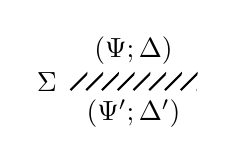
\begin{tikzpicture} 
\draw (.8,.5) node{$(\Psi; \Delta)$};
\draw (-.3, .1) node{$\Sigma$};
\draw [thick,dash pattern = on 2.82842842712mm off 2mm,decorate,decoration={saw,amplitude=2mm,segment length=2mm}] 
(0,0) -- (1.6,0); 
\draw (.8,-.3) node{$(\Psi'; \Delta')$};
\end{tikzpicture} 
\end{center}

For all process states that evolve from the initial state
$(x{:}\istrue{\susp{\sf gen}})$ under the signature $\Sigma_{\it
  Gen}$, restriction to $\Sigma_{\it PDA}$ is the identity function
whenever it is defined. Therefore, in the statement of
Theorem~\ref{thm:pda-encoding}, we use restriction as a judgment
$\restrictsig{\Delta}{\Sigma_{\it PDA}}$ that holds whenever the partial 
function is defined.

\bigskip
\begin{theorem}[Encoding]\label{thm:pda-encoding}
  Up to variable renaming, there is a bijective correspondence between
  PDA states $\obj{k \rhd s}$ and process states $\Delta$ such that
  $T :: (x{:}\istrue{\susp{\sf gen}}) \leadsto^*_{\Sigma_{\it Gen}}
  \Delta$ and $\restrictsig{\Delta}{\Sigma_{\it
      PDA}}$.
\end{theorem}

\begin{proof}To establish the bijective correspondence, we first define
an encoding function from PDA states to process states:
\smallskip
\begin{itemize}
\item $\ctxinterp{k \rhd s} = 
  \ctxinterp{k}, ~~
  h{:}\istrue{\susp{\sf hd}}, ~~
  \ctxinterp{s}$
\item $\ctxinterp{\cdot} = \cdot$
\item $\ctxinterp{k{\sf <}} = \ctxinterp{k}, ~~ x{:}\istrue{\susp{\sf <}}$
\item $\ctxinterp{{\sf <}s} = y{:}\istrue{\susp{\sf <}}, ~~ \ctxinterp{s}$
\item $\ctxinterp{{\sf >}s} = y{:}\istrue{\susp{\sf >}}, ~~ \ctxinterp{s}$
\end{itemize}
\smallskip It is always the case that $\restrictsig{\ctxinterp{k \rhd
    s}}{\Sigma_{\it PDA}}$ -- the encoding only includes terminals.
To show that the encoding function is injective we must show that, for
any $\obj{k \rhd s}$, there exists a trace $T ::
(x{:}\istrue{\susp{\sf gen}}) \leadsto^*_{\it Gen} \ctxinterp{k \rhd
  s}$. To show that the encoding function is surjective, we must show
that if $T :: (x{:}\istrue{\susp{\sf gen}}) \leadsto^*_{\Sigma_{\it
    Gen}} \Delta$ and $\restrictsig{\Delta}{\Sigma_{\it PDA}}$ then
$\Delta = \ctxinterp{k \rhd s}$ for some $\obj{k}$ and $\obj{s}$. This
will complete the proof: an injective and surjective function is
bijective.

\subsubsection{Encoding is injective}

We prove that for
any $\obj{k \rhd s}$, there exists a trace $T ::
(x{:}\istrue{\susp{\sf gen}}) \leadsto^*_{\it Gen} \ctxinterp{k \rhd
  s}$ with a series of three lemmas.

\begin{lemma} For all $\obj{k}$, there exists
$T :: ({x{:}\istrue{\susp{\sf gen\_stack}}}) \leadsto^*_{\Sigma_{\it Gen}} 
({\ctxinterp{k}, x'{:}\istrue{\susp{\sf gen\_stack}}})$.
\end{lemma}
\noindent
By induction on $\obj{k}$. 
\begin{itemize}
\item If $\obj{k} = \cdot$, $T = \emptytrace ::
({x{:}\istrue{\susp{\sf gen\_stack}}}) \leadsto^*_{\Sigma_{\it Gen}} 
(x{:}\istrue{\susp{\sf gen\_stack}})$
\item If $\obj{k} = \obj{k' {\sf <}}$, we have 
$T' :: ({x{:}\istrue{\susp{\sf gen\_stack}}}) \leadsto^*_{\Sigma_{\it Gen}} 
({\ctxinterp{k'}, x''{:}\istrue{\susp{\sf gen\_stack}}})$ by the induction
hypothesis, so $T = (T'; \trstep{x_1, x_2}{{\sf stack/left}\,x'}) :: 
({x{:}\istrue{\susp{\sf gen\_stack}}}) \leadsto^*_{\Sigma_{\it Gen}} 
({\ctxinterp{k'}, x_1{:}\istrue{\susp{\sf <}}, x_2{:}\istrue{\susp{\sf gen\_stack}}})$
\end{itemize}

\begin{lemma} For all $\obj{s}$, there exists
$T :: ({y{:}\istrue{\susp{\sf gen\_string}}}) \leadsto^*_{\Sigma_{\it Gen}} 
({x'{:}\istrue{\susp{\sf gen\_string}}, \ctxinterp{s}})$.
\end{lemma}
\noindent
By induction on $\obj{s}$.
\begin{itemize}
\item If $\obj{s} = \cdot$, $T = \emptytrace ::
({x{:}\istrue{\susp{\sf gen\_stack}}}) \leadsto^*_{\Sigma_{\it Gen}} 
(x{:}\istrue{\susp{\sf gen\_stack}})$
\item If $\obj{s} = \obj{{\sf <}s' }$, we have 
$T' :: ({x{:}\istrue{\susp{\sf gen\_string}}}) \leadsto^*_{\Sigma_{\it Gen}} 
(x'{:}\istrue{\susp{\sf gen\_string}}, \ctxinterp{s'})$ by the induction
hypothesis, so $T = (T'; \trstep{x_1, x_2}{{\sf string/left}\,x'}) :: 
({x{:}\istrue{\susp{\sf gen\_stack}}}) \leadsto^*_{\Sigma_{\it Gen}} 
(x_1{:}\istrue{\susp{\sf gen\_stack}},
 x_2{:}\istrue{\susp{\sf <}},
\ctxinterp{s'})$
\item If $\obj{s} = \obj{{\sf >}s' }$, we have 
$T' :: ({x{:}\istrue{\susp{\sf gen\_string}}}) \leadsto^*_{\Sigma_{\it Gen}} 
(x'{:}\istrue{\susp{\sf gen\_string}}, \ctxinterp{s'})$ by the induction
hypothesis, so $T = (T'; \trstep{x_1, x_2}{{\sf string/right}\,x'}) :: 
({x{:}\istrue{\susp{\sf gen\_stack}}}) \leadsto^*_{\Sigma_{\it Gen}} 
(x_1{:}\istrue{\susp{\sf gen\_stack}},
 x_2{:}\istrue{\susp{\sf >}},
\ctxinterp{s'})$
\end{itemize}

\begin{lemma} For all $\obj{k}$ and $\obj{s}$, there exists
$T :: ({g{:}\istrue{\susp{\sf gen}}}) \leadsto^*_{\Sigma_{\it Gen}} 
(\ctxinterp{k \rhd s})$. 
\end{lemma}
\noindent
By straightforward construction using the first two lemmas
and frame weakening (Theorem~\ref{thm:frameweak}): 
\begin{align*}
& \qquad\qquad (g{:}\istrue{\susp{\sf gen}})\\
& \trstep{x,h,y}{{\sf state}\,g};\\
& \qquad\qquad
       (x{:}\istrue{\susp{\sf gen\_stack}},  ~~
        h{:}\istrue{\susp{\sf hd}},~~ 
        y{:}\istrue{\susp{\sf gen\_string}})\\
& T_k; ~~ \mbox{\it (given by the first lemma and frame weakening)}\\
& \qquad\qquad
       (\ctxinterp{k},  ~~
        x'{:}\istrue{\susp{\sf gen\_stack}},  ~~
        h{:}\istrue{\susp{\sf hd}}, ~~
        y{:}\istrue{\susp{\sf gen\_string}})\\
& \trstep{()}{{\sf stack/done}\,x'}\\
& \qquad\qquad
       (\ctxinterp{k},  ~~
        h{:}\istrue{\susp{\sf hd}}, ~~
        y{:}\istrue{\susp{\sf gen\_string}})\\
& T_s; ~~ \mbox{\it (given by the second lemma and frame weakening)}\\
& \qquad\qquad
       (\ctxinterp{k}, ~~
        h{:}\istrue{\susp{\sf hd}}, ~~
        y'{:}\istrue{\susp{\sf gen\_string}}, ~~
        \ctxinterp{s})\\
& \trstep{()}{{\sf string/done}\,y'}\\
& \qquad\qquad 
       (\ctxinterp{k}, ~~
        h{:}\istrue{\susp{\sf hd}}, ~~
        \ctxinterp{s}) \\
& \qquad\qquad = \ctxinterp{k \rhd s}
\end{align*}


\subsubsection{Encoding is surjective}

We prove that if $T :: (x{:}\istrue{\susp{\sf gen}}) \leadsto^*_{\Sigma_{\it
    Gen}} \Delta$ and $\restrictsig{\Delta}{\Sigma_{\it PDA}}$ then
$\Delta = \ctxinterp{k \rhd s}$ for some $\obj{k}$ and $\obj{s}$
any $\obj{k \rhd s}$, there exists a trace $T ::
(x{:}\istrue{\susp{\sf gen}}) \leadsto^*_{\it Gen} \ctxinterp{k \rhd
  s}$ with a series of two lemmas.

\begin{lemma} If 
$T :: (\ctxinterp{k}, 
       x{:}\istrue{\susp{\sf gen\_stack}}, 
       h{:}\istrue{\susp{\sf hd}},
       y{:}\istrue{\susp{\sf gen\_store}},
       \ctxinterp{s}) 
  \leadsto^*_{\Sigma_{\it Gen}} \Delta$ and
$\restrictsig{\Delta}{\Sigma_{\it
      PDA}}$, then $\Delta = \ctxinterp{k' \rhd s'}$ for some $\obj{k'}$
and $\obj{s'}$.
\end{lemma}
\noindent
By induction on the structure of $T$ and case analysis on the 
first steps in $T$. Up to concurrent equality, there
are four possibilities:
\smallskip
\begin{itemize}
\item $T = (\trstep{()}{{\sf stack/done}\,x}; \trstep{()}{{\sf
      state/done}\,y})$ -- this is a base case, and we can finish by
  letting $\obj{k'} = \obj{k}$ and $\obj{s'} = \obj{s}$.
\item $T = (\trstep{x_1,x_2}{{\sf stack/left}\,x}; T')$ -- apply 
  the ind.~hyp.~(letting $x = x_2$, $\obj{k} =
  \obj{k{\sf <}}$).
\item $T = (\trstep{y_1,y_2}{{\sf string/left}\,y}; T')$ -- apply
  the ind.~hyp.~(letting $y = y_1$, $\obj{s} =
  \obj{{\sf <}s}$).
\item $T = (\trstep{y_1,y_2}{{\sf string/right}\,y}; T')$ -- apply
  the ind.~hyp.~(letting $y = y_1$, $\obj{s} =
  \obj{{\sf >}s}$).
\end{itemize}
\smallskip 
The proof above takes
a number of facts about concurrent equality for granted. 
%
For example, the trace $T = (\trstep{()}{{\sf stack/done}\,x};
\trstep{y_1,y_2}{{\sf string/right}\,y}; T')$ does not syntactically
match any of the traces above if we do not account for concurrent
equality. Modulo concurrent equality, on the other hand, $T =
(\trstep{y_1,y_2}{{\sf string/right}\,y}; \trstep{()}{{\sf
    stack/done}\,x}; T')$, matching the last branch of the case
analysis.  If we didn't implicitly rely on concurrent equality in this
way, the resulting proof would have twice as many cases.  We will take
these finite uses of concurrent equality for granted when we specify
that a proof proceeds by case analysis on the first steps of $T$ (or,
conversely, by case analysis on the last steps of $T$).

\begin{lemma} If 
$T :: (g{:}\istrue{\susp{\sf gen}}) 
  \leadsto^*_{\Sigma_{\it Gen}} \Delta$ and
$\restrictsig{\Delta}{\Sigma_{\it
      PDA}}$, then $\Delta = \ctxinterp{k' \rhd s'}$ for some $\obj{k'}$
and $\obj{s'}$.
\end{lemma}
\noindent
This is a corollary of the previous lemma, as it can only
be the case that $T = \trstep{x,h,y}{{\sf state}\,g}; T'$. We can apply the previous
lemma to $T'$, letting $\obj{k} = \obj{s} = \obj{\cdot}$.
This establishes that encoding is a surjective function, which in turn
completes the proof. 
\end{proof}

Theorem~\ref{thm:pda-encoding} establishes that the generative
signature $\Sigma_{\it Gen}$ describes a world -- a set of
\sls~process states -- that precisely correspond to the states of a
push-down automata.  We can (imperfectly) illustrate the content of
this theorem in our two-dimensional notation as follows, where 
$\Delta \Leftrightarrow \obj{k \rhd s}$ indicates the presence of a
bijection:
\begin{center}
\begin{tikzpicture} 
\draw (.8,2.3) node{$(x{:}\istrue{\susp{\sf gen}})$};
\draw [->,decorate, 
decoration={snake,amplitude=.3mm,segment length=3mm,post length=1mm}] 
(0.8,2) -- (.8,.8); 
\draw (.9,.8) node{$_*$};
\draw (.3,1.4) node{$\Sigma_{\it Gen}$};
\draw (.8,.5) node{$\Delta$};
\draw (-.2, .1) node{$\Sigma_{\it PDA}$};
\draw [thick,dash pattern = on 2.82842842712mm off 2mm,decorate,decoration={saw,amplitude=2mm,segment length=2mm}] 
(.4,0) -- (1.2,0); 
\draw (.8,-.3) node{$\Delta$};
\draw (1.1,-.7) node{\begin{turn}{-45}$\Leftrightarrow$\end{turn}};
\draw (1.8,-1) node{$\obj{k \rhd s}$};
\end{tikzpicture} 
\end{center}

It is interesting to note how the proof of
Theorem~\ref{thm:pda-encoding} takes advantage of the associative
structure of traces: the inductive process that constructed traces in
the first two lemmas treated trace composition as left-associative,
but the induction we performed on traces in the next-to-last lemma
treated trace composition as right-associative.

\subsection{Generated world preservation}

The generative signature $\Sigma_{\it Gen}$ precisely captures the
world of \sls~process states that are in the image of the encoding
$\ctxinterp{k \rhd s}$ of PDA states as process states. In order for
the signature $\Sigma_{\it PDA}$ to encode a reasonable notion of
transition between PDA states, we need to show that steps in this
signature only take encoded PDA states to encoded PDA states. Because 
the generative signature $\Sigma_{\it Gen}$ precisely captures the 
process states that represent encoded PDA states, we can describe
and prove this property without reference to the actual encoding function:
 
\bigskip
\begin{theorem}[Preservation]\label{thm:pda-preservation}
If $T_1 :: (x{:}\istrue{\susp{\sf gen}}) \leadsto^*_{\Sigma_{\it Gen}} \Delta_1$,
$\restrictsig{\Delta_1}{\Sigma_{\it PDA}}$, and 
$S :: \Delta_1 \leadsto_{\Sigma_{\it PDA}} \Delta_2$, then 
$T_2 :: (x{:}\istrue{\susp{\sf gen}}) \leadsto^*_{\Sigma_{\it Gen}} \Delta_2$.
\end{theorem}
\bigskip

\noindent
If we illustrate given elements as solid lines and elements that we have
to prove as dashed lines, the big picture of the encoding and preservation
theorems is the following:

\begin{center}
\begin{tikzpicture} 
\draw (.8,2.3) node{$(x{:}\istrue{\susp{\sf gen}})$};
\draw [->,decorate, 
decoration={snake,amplitude=.3mm,segment length=3mm,post length=1mm}] 
(0.8,2) -- (.8,.8); 
\draw (.9,.8) node{$_*$};
\draw (.3,1.4) node{$\Sigma_{\it Gen}$};
\draw (.8,.5) node{$\Delta$};
\draw [thick,dash pattern = on 2.82842842712mm off 2mm,decorate,decoration={saw,amplitude=2mm,segment length=2mm}] 
(.4,0) -- (1.2,0); 
\draw (.8,-.3) node{$\Delta$};
\draw (1.1,-.7) node{\begin{turn}{-45}$\Leftrightarrow$\end{turn}};
\draw (1.8,-1) node{$\obj{k \rhd s}$};
%
\draw (4.8,2.3) node{$(x{:}\istrue{\susp{\sf gen}})$};
\draw [->,densely dotted,decorate, 
decoration={snake,amplitude=.3mm,segment length=3mm,post length=1mm}] 
(4.8,2) -- (4.8,.8); 
\draw (4.9,.8) node{$_*$};
\draw (4.3,1.4) node{$\Sigma_{\it Gen}$};
\draw (4.8,.5) node{$\Delta'$};
\draw (2.8, 0) node{$\Sigma_{\it PDA}$};
\draw [thick,dash pattern = on 0.677mm off .4mm on 0.676142375mm off .4mm on 0.676142375mm off 2mm,decorate,decoration={saw,amplitude=2mm,segment length=2mm}] 
(4.4,0) -- (5.2,0); 
\draw (4.8,-.3) node{$\Delta'$};
\draw (5.1,-.7) node{\begin{turn}{-45}$\Leftrightarrow$\end{turn}};
\draw (5.8,-1) node{$\obj{k' \rhd s'}$};
%
\draw [->,decorate, 
decoration={snake,amplitude=.3mm,segment length=3mm,post length=1mm}] 
(1.2,-.3) -- (4.4,-.3); 
\end{tikzpicture} 
\end{center}

\noindent
The proof of Theorem~\ref{thm:pda-preservation} relies on two lemmas, 
which we will consider before the proof itself. They are both
{\it inversion lemmas}: they help uncover the structure of the
trace based on the type of that trace. Treating
traces modulo concurrent equality is critical in both cases. 

\bigskip
\begin{lemma}
  Let $\Delta = \tackon{\Theta}{x{:}\istrue{\susp{\sf gen\_stack}},
    h{:}\istrue{\susp{\sf hd}}, y{:}\istrue{\susp{\sf gen\_state}}}$.
  If $T :: \Delta \leadsto^*_{\Sigma_{\it Gen}} \Delta'$ and
  $\restrictsig{\Delta'}{\Sigma_{\it PDA}}$, then $T = (T';
  \trstep{()}{{\sf stack/done}\,x}; \trstep{()}{{\sf
      string/done}\,y})$, where $T' ::
  \Delta \leadsto^*_{\Sigma_{\it Gen}}
  \tackon{\Theta'}{x'{:}\istrue{\susp{\sf gen\_stack}},
    h{:}\istrue{\susp{\sf hd}}, y'{:}\istrue{\susp{\sf gen\_state}}}$
  and $\Delta' = \tackon{\Theta'}{h{:}\istrue{\susp{\sf hd}}}$.
\end{lemma}
\begin{proof}
By induction on the structure of $T$ and case analysis on the first
steps in $T$. Up to concurrent equality, there are five possibilities:
\begin{itemize}
\item $T = (\trstep{()}{{\sf stack/done}\,x}; \trstep{()}{{\sf
      string/done}\,y})$. Immediate, letting $T' = \emptytrace$.
\item $T = (\trstep{x_1,x_2}{{\sf stack/left}\,x}; T'')$. By the
  induction hypothesis (where the new frame incorporates
  $x_1{:}\istrue{\susp{\sf <}}$), we have $T'' = (T''';
  \trstep{()}{{\sf stack/done}\,x}; \trstep{()}{{\sf
      string/done}\,y})$. Let $T' = (\trstep{x_1,x_2}{{\sf
      stack/left}\,x}; T''')$.
\item $T = (\trstep{y_1,y_2}{{\sf string/left}\,y}; T'')$. By the
  induction hypothesis (where the new frame incorporates
  $y_1{:}\istrue{\susp{\sf <}}$), we have $T'' = (T''';
  \trstep{()}{{\sf stack/done}\,x}; \trstep{()}{{\sf
      string/done}\,y})$. Let $T' = (\trstep{x_1,x_2}{{\sf
      string/left}\,y}; T''')$.
\item $T = (\trstep{y_1,y_2}{{\sf string/right}\,y}; T'')$. By the
  induction hypothesis (where the new frame incorporates
  $y_2{:}\istrue{\susp{\sf >}}$), we have $T'' = (T''';
  \trstep{()}{{\sf stack/done}\,x}; \trstep{()}{{\sf
      string/done}\,y})$. Let $T' = (\trstep{x_1,x_2}{{\sf
      string/right}\,y}; T''')$.
\item $T = (S; T'')$, where $x$ and $y$ are not free in $S$. 
      By the induction hypothesis, we have
      $T'' = (T''';
       \trstep{()}{{\sf stack/done}\,x}; \trstep{()}{{\sf
       string/done}\,y})$. Let $T' = (S; T''')$. (This case will not arise
      in the way we use this lemma, but the statement of the theorem 
      leaves open the possibility that there are other nonterminals
      in $\Theta$.)
\end{itemize}
This completes the proof. 
\end{proof}

A corollary of this lemma is that if 
$T :: (g{:}\istrue{\susp{\sf gen}}) \leadsto^*_{\Sigma_{\it Gen}} \Delta$ and
  $\restrictsig{\Delta}{\Sigma_{\it PDA}}$, then $T = (T';
  \trstep{()}{{\sf stack/done}\,x}; \trstep{()}{{\sf
      string/done}\,y})$ -- modulo concurrent equality, naturally -- 
where $T' ::
  (g{:}\istrue{\susp{\sf gen}}) \leadsto^*_{\Sigma_{\it Gen}}
  \tackon{\Theta}{x'{:}\istrue{\susp{\sf gen\_stack}},
    h{:}\istrue{\susp{\sf hd}}, y'{:}\istrue{\susp{\sf gen\_state}}}$
  and $\Delta = \tackon{\Theta}{h{:}\istrue{\susp{\sf hd}}}$. To prove
the corollary, we observe
that $T = (\trstep{x,h,r}{{\sf state}\,g\,}; T'')$ and apply the lemma
to $T''$. 

\bigskip
\begin{lemma} The following all hold:
\begin{itemize}
\item If $T :: (g{:}\istrue{\susp{\sf gen}}) \leadsto^*_{\Sigma_{\it Gen}} 
       \tackon{\Theta}{x_1{:}\istrue{\susp{\sf <}}, 
          x_2{:}\istrue{\susp{\sf gen\_stack}}}$, \\then 
$T = (T'; \trstep{x_1,x_2}{{\sf stack/left}\,x'})$. 
\item If $T :: (g{:}\istrue{\susp{\sf gen}}) \leadsto^*_{\Sigma_{\it Gen}} 
       \tackon{\Theta}{y_1{:}\istrue{\susp{\sf gen\_stack}},
           y_2{:}\istrue{\susp{\sf <}}}$, \\then 
$T = (T'; \trstep{x_1,x_2}{{\sf string/left}\,y'})$. 
\item If $T :: (g{:}\istrue{\susp{\sf gen}}) \leadsto^*_{\Sigma_{\it Gen}} 
       \tackon{\Theta}{y_1{:}\istrue{\susp{\sf gen\_stack}},
           y_2{:}\istrue{\susp{\sf >}}}$, \\then 
$T = (T'; \trstep{x_1,x_2}{{\sf string/right}\,y'})$. 
\end{itemize}
\end{lemma}
\begin{proof}
The proofs are all by induction on the structure of $T$ and case
analysis on the last steps in $T$; we will prove the last statement, as
the other two are similar. Up to concurrent equality, there are two
possibilities:
\begin{itemize}
\item $T = (T'; \trstep{y_1, y_2}{{\sf string/right}\,y'})$ -- Immediate.
\item $T = (T''; S)$, where $y_1$ and $y_2$ are not bound by $S$. By the 
induction hypothesis, $T'' = (T'''; \trstep{y_1,y_2}{{\sf string/right}\,y'})$.
Let $T' = (T''; S)$. 
\end{itemize}
This completes the proof. 
\end{proof}

Note that we do not consider any cases where 
$T = (T'; \trstep{y_1',y_2}{{\sf string/right}\,y'})$ (for $y_1 \neq y_1'$),
$T = (T'; \trstep{y_1',y_2}{{\sf string/right}\,y'})$ (for $y_2 \neq y_2'$),
or (critically) where 
$T = (T'; \trstep{y_1,y_2'}{{\sf string/left}\,y'})$. There is no 
way for any of these traces to have the correct type, which makes
the resulting case analysis quite simple. 

\begin{proof}[Proof of Theorem~\ref{thm:pda-preservation} (Preservation)]
By case analysis on the structure of $S$. 

\bigskip
\noindent
{\bf Case 1:} $S = \trstep{x',h'}{{\sf push}\,(\tfuser{h}{y})}$,
which means that we are given the following 
generative trace in $\Sigma_{\it Gen}$:
\begin{align*}
& \qquad ({g{:}\istrue{\susp{\sf gen}}})\\
& T\\
& \qquad \tackon{\Theta}{h{:}\istrue{\susp{\sf hd}}, ~~
                   y{:}\istrue{\susp{\sf <}}}
\intertext{and we must construct a trace 
$({g{:}\istrue{\susp{\sf gen}}}) \leadsto^*_{\Sigma_{\it Gen}} 
\tackon{\Theta}{x'{:}\istrue{\susp{\sf <}},
                   h'{:}\istrue{\susp{\sf hd}}}$. Changing
$h$ to $h'$ is just renaming a bound variable, so we have}
& \qquad 
({g{:}\istrue{\susp{\sf gen}}})\\
& T'\\
& \qquad \tackon{\Theta}{h'{:}\istrue{\susp{\sf hd}}, ~~
                   y{:}\istrue{\susp{\sf <}}}
\intertext{
The corollary 
to the first inversion lemma above on $T'$ gives us}
T' = & \qquad 
({g{:}\istrue{\susp{\sf gen}}})\\
& T'';\\
& \qquad \tackon{\Theta}{
                   x_g{:}\istrue{\susp{\sf gen\_stack}}, ~~
                   h'{:}\istrue{\susp{\sf hd}}, ~~
                   y_g{:}\istrue{\susp{\sf gen\_string}}, ~~
                   y{:}\istrue{\susp{\sf <}}}\\
& \trstep{()}{{\sf stack/done}\,x_g};\\
& \trstep{()}{{\sf string/done}\,y_g}\\
& \qquad \tackon{\Theta}{h'{:}\istrue{\susp{\sf hd}}, ~~
                   y{:}\istrue{\susp{\sf <}}}
\intertext{The second inversion lemma (second part) on $T''$ gives us}
T'' = & \qquad 
({g{:}\istrue{\susp{\sf gen}}})\\
& T''';\\
& \qquad \tackon{\Theta}{
                   x_g{:}\istrue{\susp{\sf gen\_stack}}, ~~
                   h'{:}\istrue{\susp{\sf hd}}, ~~
                   y_g'{:}\istrue{\susp{\sf gen\_string}}}\\
& \trstep{y_g,y}{{\sf string/left}\,y_g'};\\
& \qquad \tackon{\Theta}{
                   x_g{:}\istrue{\susp{\sf gen\_stack}}, ~~
                   h'{:}\istrue{\susp{\sf hd}}, ~~
                   y_g{:}\istrue{\susp{\sf gen\_string}}, ~~
                   y{:}\istrue{\susp{\sf <}}}\\
\intertext{Now, we can construct the trace we need using $T'''$:}
& \qquad 
({g{:}\istrue{\susp{\sf gen}}})\\
& T''';\\
& \qquad \tackon{\Theta}{
                   x_g{:}\istrue{\susp{\sf gen\_stack}}, ~~
                   h'{:}\istrue{\susp{\sf hd}}, ~~
                   y_g'{:}\istrue{\susp{\sf gen\_string}}}\\
& \trstep{x', x_g'}{{\sf stack/left}\,x_g};\\
& \qquad \tackon{\Theta}{
                   x'{:}\istrue{\susp{\sf <}}, ~~
                   x_g'{:}\istrue{\susp{\sf gen\_stack}}, ~~
                   h'{:}\istrue{\susp{\sf hd}}, ~~
                   y_g'{:}\istrue{\susp{\sf gen\_string}}}\\
& \trstep{()}{{\sf stack/done}\,x_g'};\\
& \trstep{()}{{\sf string/done}\,y_g'}\\
& \qquad \tackon{\Theta}{
                   x'{:}\istrue{\susp{\sf <}}, ~~
                   h'{:}\istrue{\susp{\sf hd}}}
\end{align*}

\bigskip
\noindent
{\bf Case 2:} $S = \trstep{h'}{{\sf pop}\,(\tfuser{x}{\tfuser{h}{y}})}$,
which means that we are given the following 
generative trace in $\Sigma_{\it Gen}$:
\begin{align*}
& \qquad ({g{:}\istrue{\susp{\sf gen}}})\\
& T\\
& \qquad \tackon{\Theta}{x{:}\istrue{\susp{\sf <}}, ~~
                   h{:}\istrue{\susp{\sf hd}}, ~~
                   y{:}\istrue{\susp{\sf >}}}
\intertext{and we must construct a trace 
$({g{:}\istrue{\susp{\sf gen}}}) \leadsto^*_{\Sigma_{\it Gen}} 
\tackon{\Theta}{h'{:}\istrue{\susp{\sf hd}}}$. Changing
$h$ to $h'$ is just renaming a bound variable, so we have}
& \qquad ({g{:}\istrue{\susp{\sf gen}}})\\
& T'\\
& \qquad \tackon{\Theta}{x{:}\istrue{\susp{\sf <}}, ~~
                   h'{:}\istrue{\susp{\sf hd}}, ~~
                   y{:}\istrue{\susp{\sf >}}}
\intertext{The corollary to the first inversion lemma above on $T'$ gives us}
T' = & \qquad ({g{:}\istrue{\susp{\sf gen}}})\\
& T'';\\
& \qquad \tackon{\Theta}{x{:}\istrue{\susp{\sf <}}, ~~
                   x_g{:}\istrue{\susp{\sf gen\_stack}}, ~~
                   h'{:}\istrue{\susp{\sf hd}}, ~~
                   y_g{:}\istrue{\susp{\sf gen\_string}}, ~~
                   y{:}\istrue{\susp{\sf >}}}\\
& \trstep{()}{{\sf stack/done}\,x_g};\\
& \trstep{()}{{\sf string/done}\,y_g}\\
& \qquad \tackon{\Theta}{x{:}\istrue{\susp{\sf <}}, ~~
                   h'{:}\istrue{\susp{\sf hd}}, ~~
                   y{:}\istrue{\susp{\sf >}}}
\intertext{The second inversion lemma (first part) on $T''$ gives us}
T'' = & \qquad ({g{:}\istrue{\susp{\sf gen}}})\\
& T''';\\
& \qquad \tackon{\Theta}{x_g'{:}\istrue{\susp{\sf gen\_stack}}, ~~
                   h'{:}\istrue{\susp{\sf hd}}, ~~
                   y_g{:}\istrue{\susp{\sf gen\_string}}, ~~
                   y{:}\istrue{\susp{\sf >}}}\\
& \trstep{x, x_g}{{\sf stack/left}\,x_g'};\\
& \qquad \tackon{\Theta}{x{:}\istrue{\susp{\sf <}}, ~~
                   x_g{:}\istrue{\susp{\sf gen\_stack}}, ~~
                   h'{:}\istrue{\susp{\sf hd}}, ~~
                   y_g{:}\istrue{\susp{\sf gen\_string}}, ~~
                   y{:}\istrue{\susp{\sf >}}}\\
\intertext{The second inversion lemma (third part) on $T'''$ gives us}
T''' = & \qquad ({g{:}\istrue{\susp{\sf gen}}})\\
& T'''';\\
& \qquad \tackon{\Theta}{x_g'{:}\istrue{\susp{\sf gen\_stack}}, ~~
                   h'{:}\istrue{\susp{\sf hd}}, ~~
                   y_g'{:}\istrue{\susp{\sf gen\_string}}}\\
& \trstep{y_g, y}{{\sf string/right}\,y_g'};\\
& \qquad \tackon{\Theta}{x_g'{:}\istrue{\susp{\sf gen\_stack}}, ~~
                   h'{:}\istrue{\susp{\sf hd}}, ~~
                   y_g{:}\istrue{\susp{\sf gen\_string}}, ~~
                   y{:}\istrue{\susp{\sf >}}}\\
\intertext{Now, we can construct the trace we need using $T''''$:}
& \qquad ({g{:}\istrue{\susp{\sf gen}}})\\
& T'''';\\
& \qquad \tackon{\Theta}{x_g'{:}\istrue{\susp{\sf gen\_stack}}, ~~
                   h'{:}\istrue{\susp{\sf hd}}, ~~
                   y_g'{:}\istrue{\susp{\sf gen\_string}}}\\
& \trstep{()}{{\sf stack/done}\,x_g'};\\
& \trstep{()}{{\sf string/done}\,y_g'}\\
& \qquad \tackon{\Theta}{h'{:}\istrue{\susp{\sf hd}}}
\end{align*}

\noindent
These two cases represent the only two synthetic transitions that are possible
under the signature $\Sigma_{\it PDA}$, so we are done.
\end{proof}

Proving that generation under a generative signature like $\Sigma_{\it
  Gen}$ is invariant under transitions in a signature like
$\Sigma_{\it PDA}$ is something we will consider further
in Chapter 9.  All such proofs essentially follow the structure of
Theorem~\ref{thm:pda-preservation}. First, we enumerate the synthetic
transitions associated with a given signature. Second, in each of those
cases, we use the type of the synthetic transition to perform
inversion on the structure of the given generative trace.
Third, we construct a generative
trace that establishes the fact that the invariant was preserved.

\subsection{Adequacy for LF and deductive terms}

The hard work of adequacy is established by the preservation theorem; 
the actual adequacy theorem is just an enumeration in both directions.

\bigskip
\begin{theorem}[Adequacy]\label{thm:pda-adequacy}
  $\ctxinterp{k \rhd s} \leadsto^*_{\Sigma_{\it PDA}} \ctxinterp{k'
    \rhd s'}$ if and only if $\obj{k \rhd s} \mapsto \obj{k' \rhd s'}$.
\end{theorem}

\begin{proof}
  Both directions can be established by case analysis on the structure
  of $\obj{k}$ and $\obj{s}$.
\end{proof}

In our two-dimensional notation, the complete discussion of adequacy
for \sls~is captured by the following picture:

\begin{center}
\begin{tikzpicture} 
\draw (.8,2.3) node{$(x{:}\istrue{\susp{\sf gen}})$};
\draw [->,decorate, 
decoration={snake,amplitude=.3mm,segment length=3mm,post length=1mm}] 
(0.8,2) -- (.8,.8); 
\draw (.9,.8) node{$_*$};
\draw (.3,1.4) node{$\Sigma_{\it Gen}$};
\draw (.8,.5) node{$\Delta$};
\draw [thick,dash pattern = on 2.82842842712mm off 2mm,decorate,decoration={saw,amplitude=2mm,segment length=2mm}] 
(.4,0) -- (1.2,0); 
\draw (.8,-.3) node{$\Delta$};
\draw (1.1,-.7) node{\begin{turn}{-45}$\Leftrightarrow$\end{turn}};
\draw (1.8,-1) node{$\obj{k \rhd s}$};
%
\draw (4.8,2.3) node{$(x{:}\istrue{\susp{\sf gen}})$};
\draw [->,densely dotted,decorate, 
decoration={snake,amplitude=.3mm,segment length=3mm,post length=1mm}] 
(4.8,2) -- (4.8,.8); 
\draw (4.9,.8) node{$_*$};
\draw (4.3,1.4) node{$\Sigma_{\it Gen}$};
\draw (4.8,.5) node{$\Delta'$};
\draw (2.8, 0) node{$\Sigma_{\it PDA}$};
\draw [thick,dash pattern = on 0.677mm off .4mm on 0.676142375mm off .4mm on 0.676142375mm off 2mm,decorate,decoration={saw,amplitude=2mm,segment length=2mm}] 
(4.4,0) -- (5.2,0); 
\draw (4.8,-.3) node{$\Delta'$};
\draw (5.1,-.7) node{\begin{turn}{-45}$\Leftrightarrow$\end{turn}};
\draw (5.8,-1) node{$\obj{k' \rhd s'}$};
%
\draw [->,decorate, 
decoration={snake,amplitude=.3mm,segment length=3mm,post length=1mm}] 
(1.2,-.3) -- (4.4,-.3); 
\draw [|->] (2.5,-1.04) -- (5,-1.04);;
\end{tikzpicture} 
\end{center}

\section{The \sls~implementation}
\label{sec:prototype}

The prototype implementation of \sls~contains a parser and typechecker
for the SLS language, and is available from
\url{https://github.com/robsimmons/sls}. Code that is checked by this
prototype implementation will appear frequently in the rest of this
thesis, always in a \verb|fixed-width font|.

\begin{figure}
\newcommand{\thingamajig}{=}
\begin{align*}
{\downarrow}A^- & \thingamajig \mbox{\Verb|A|} 
 & {\ocircle}A^+ & \thingamajig \mbox{\Verb|\{A\}|}
 & \lf{\lambda a.t} & \thingamajig \mbox{{\texttt{\char`\\}}\Verb|a.t|}
\\
{\gnab}A^- & \thingamajig \mbox{\Verb|\$A|}
 & A^+ \lefti B^- & \thingamajig \mbox{\Verb|A >-> B|}
 & \lf{{\sf foo}\,t_1\ldots t_n} & \thingamajig \mbox{\Verb|foo t1...tn|}
\\
{!}A^- & \thingamajig \mbox{\Verb|!A|}
 & A^+ \righti B^- & \thingamajig \mbox{\Verb|A ->> B|}
\\
\one & \thingamajig \mbox{\Verb|one|}
 & A^- \with B^- & \thingamajig \mbox{\Verb|A \& B|}
 & \Pi\lf{a}{:}\tau.\nu & \thingamajig \mbox{\Verb|Pi x.nu|}
\\
A^+ \fuse B^+ & \thingamajig \mbox{\Verb|A * B|}
 & \forall \lf{a}.\tau. A^- & \thingamajig \mbox{\Verb|All x.A|}
 & \tau \rightarrow \nu & \thingamajig{\mbox{\Verb|tau -> nu|}}
\\
\exists \lf{a}.\tau. A^+ & \thingamajig \mbox{\Verb|Exists x.A|}
 & {\gnab}A^- \lefti B^- & \thingamajig \mbox{\Verb|A -o B|}
 & {\sf bar}\,\lf{t_1 \ldots t_n} & \thingamajig{\mbox{\Verb|bar t1...tn|}}
\\
\lf{t} \doteq \lf{s} & \thingamajig \mbox{\Verb|t == s|}
 & {!}A^- \lefti B^- & \thingamajig \mbox{\Verb|A -> B|}
\end{align*}
\caption{Mathematical and ASCII representations of propositions,
  terms, and classifiers}
\label{fig:translate-types}
\end{figure}


The checked \sls~code differs slightly from mathematical \sls~code in
a few ways -- the
translation between the mathematical notation we use for
\sls~propositions and the ASCII representation used in the
implementation is outlined in Figure~\ref{fig:translate-types}.
Following CLF and the Celf implementation, we write the
lax modality ${\ocircle}A$ in ASCII as \verb|{A}| -- recall that in
Section~\ref{sec:slsframework} we introduced the $\{ A^+ \}$ notation
from CLF as a synonym for Fairtlough and Mendler's ${\ocircle}A^+$.
The exponential ${\gnab}A$ doesn't have an ASCII
representation, so write \verb|$A| when $A$ is mobile. Upshifts and
downshifts are always inferred: this means that we can't write down
${\uparrow}{\downarrow}A$ or ${\downarrow}{\uparrow}A$, but neither of
these \ollll~propositions are part of the \sls~fragment anyway. 

The \sls~implementation also supports conventional abbreviations for
arrows that we will won't use in mathematical notation: ${\gnab}A^-
\lefti B^-$ can be written as \verb|A -o B| or \verb|$A >-> B| in the
\sls~implementation, and ${!}A^- \lefti B^-$ can be written as
\verb|A -> B| or \verb|!A >-> B|.  (This final proposition is
ambiguous, because \verb|X -> Y| can be an abbreviation for ${!}X
\lefti Y$ or $\Pi \lf{a}{:}X. Y$, but \sls~can figure out whether the
proposition or classifier was intended by analyzing the structure of
\verb|Y|.)  All arrows can also be written backwards: \verb|B <-< A|
is equivalent to \verb|A >-> B|, \verb|B o- A| is equivalent to
\verb|A -o B|, and so on. Also following traditional conventions,
upper-case variables that are free in a rule will be treated as
implicitly quantified. Therefore, the line
\bigskip
\begin{verbatim}
rule: foo X <- (bar Y -> baz Z).
\end{verbatim}
\bigskip
will be reconstructed as the \sls~declaration 
\[{\sf rule} : \forall\lf{Y}{:}\tau_1.\,\forall\lf{Z}{:}\tau_2.\,\forall\lf{X}{:}\tau_3.\,{!}({!}{\sf bar}\,\lf{Y} \lefti {\sf baz}\,\lf{Z}) \lefti {\sf foo}\,\lf{X}\] 
%
where the implementation infers the types $\tau_1$, $\tau_2$, and
$\tau_3$ appropriately from the declarations of the negative
predicates ${\sf foo}$, ${\sf bar}$, and ${\sf baz}$.

Another significant piece of syntactic sugar introduced for 
the sake of readability is less conventional, if only because
positive atomic propositions are not conventional. If \verb|P| is a
persistent atomic proposition, we can optionally write \verb|!P|
wherever \verb|P| is expected, and if \verb|P| is a linear atomic
proposition, we can write \verb|$P| wherever \verb|P| is
expected. This means that if ${\sf a}$, ${\sf b}$, and ${\sf c}$ are
(respectively) ordered, linear, and persistent positive atomic
propositions, we can write the positive proposition ${\sf a} \fuse
{\sf b} \fuse {\sf c}$ in the \sls~implementation as
\verb|(a * b * c)|, \verb|(a * $b * c)|, \verb|(a * b * !c)|, or
\verb|(a * $b * !c)|. Without these annotations, it is difficult to
tell at a glance which propositions are ordered, linear, or persistent
when a signature uses more than one proposition. When all of these
optional annotations are included, the rules in a signature that uses
positive atomic propositions look the same as rules in a signature
that uses the pseudo-positive negative atomic propositions described
in Section~\ref{sec:pseudopositive}. 


In the code examples given in the remainder of this thesis, we will
use these optional annotations in a consistent way.  We will omit the
optional \verb|$A| annotations only in specifications with no ordered
atomic propositions, and we will omit the optional \verb|!A|
annotations in specifications with no ordered or linear atomic
propositions. This makes the mixture of different exponentials
explicit while avoiding the need for rules like
\verb|($a * $b * $c >-> {$d * $e})| when specifications are entirely
linear (and likewise when specifications are entirely persistent).

\section{Logic programming}
\label{sec:framework-logicprog}

One logic programming interpretation of CLF was explored by the
Lollimon implementation \cite{lopez05monadic} and adapted by the Celf
implementation \cite{schacknielsen08celf}. Logic programming
interpretations of \sls~are not a focus this thesis, but we will touch
on a few points in this section. 

Logic programming is important because it provides us with operational
intuitions about the intended behavior of the systems we specify in
\sls. One specific set of these intuitions will form the basis of the
operationalization transformations on \sls~specifications considered
in Chapter~6. Additionally, logic programming intuitions are relevant
because they motivated the design of \sls, in particular the
presentation of the concurrent fragment in terms of partial, rather
than complete, proofs. We discuss this point in
Section~\ref{sec:framework-logicprog-trace}.

\subsection{Deductive computation and backward chaining}
\label{sec:framework-logicprog-deductive}
\label{sec:framework-modes}

Deductive computation in \sls~is the search for {\it complete} proofs
of sequents of the form $\foc{\Psi}{\Delta}{\istrue{\susp{p^-}}}$.  A
common form of deductive computation is {\it goal-directed search}, or
what Andreoli calls the {\it proof construction paradigm}
\cite{andreoli01focussing}.
In \sls, goal-directed search for the proof of a sequent
$\foc{\Psi}{\Delta}{\istrue{\susp{p^-}}}$ can only proceed by focusing
on a proposition like ${\downarrow}p_n^- \lefti \ldots \lefti
{\downarrow}p_1^- \lefti p^-$ which has a head $p^-$ that matches the
succedent. This replaces the goal sequent
$\foc{\Psi}{\Delta}{\istrue{\susp{p^-}}}$ with $n$ subgoals:
$\foc{\Psi}{\Delta_1}{\istrue{\susp{p_1^-}}}$ \ldots
$\foc{\Psi}{\Delta_n}{\istrue{\susp{p_n^-}}}$, where $\Delta$ matches
$\Delta_1,\ldots,\Delta_n$.

When goal-directed search only tries to build one derivation at a
time, it is called {\it backward chaining}, because we're working
backwards from the goal we want to prove.\footnote{The alternative is
  to try and derive the same sequent in multiple ways simultaneously,
  succeeding whenever some way of proving the sequent is
  discovered. Unlike backward chaining, this strategy of breadth-first
  search is complete: if a proof exists, it will be found.  Backward
  chaining as we define it is only nondeterministically or 
  partially complete,
  because it can fail to terminate when a proof exists. We will call
  this alternative to backtracking {\it breadth-first theorem
    proving}, as it amounts to taking a breadth-first, instead of
  depth-first, view of the so-called {\it failure continuation}
  \cite{pfenning06backtracking}.} The term {\it top-down logic
  programming} is also used, and refers to the fact that, in the
concrete syntax of Prolog, the rule ${\downarrow}p_n^- \lefti \ldots
\lefti {\downarrow}p_1^- \lefti p^-$ would be written with $p^-$ on
the first line, $p_1^-$ on the second, etc. This is exactly backwards
from a proof-construction perspective, as we think of backward
chaining as building partial proofs from the bottom up, the
root towards the leaves, so we will
avoid this terminology.  

The backward-chaining interpretation of intuitionistic logics dates
back to the work by Miller et al.~on uniform proofs
\cite{miller91uniform}.  An even older concept, Clark's {\it
  negation-as-failure} \cite{clark87negation}, is based on a {\it
  partial completeness} criteria for logic programming interpreters.
Partial soundness (or partial correctness) demands that if the
interpreter reports that it has found a proof of a goal-directed
sequent, such a proof should exist. Partial completeness, on the other
hand, demands that if the interpreter gives up up on finding a proof,
no proof should exist. (The interpreter is also allowed to run forever
without succeeding or giving up.)  Partial completeness requires {\it
  backtracking} in backward-chaining search: if we we try to prove
$\foc{\Psi}{\Delta}{\istrue{\susp{p^-}}}$ by focusing on a particular
proposition and one of the resulting subgoals fails to be provable, we
have to consider any other propositions that could have been used to
prove the sequent before giving up. Backtracking can be extremely
powerful in certain cases and incredibly expensive in others, and so
most logic programming languages have an escape hatch that modifies or
limits backtracking at the user's discretion, such as the Prolog cut
(no relation to the admissible rule ${\it cut}$) or Twelf's
deterministic declarations. Non-backtracking goal-oriented deductive
computation is called {\it flat resolution} \cite{aitkaci99warrens}.

One feature of backward chaining and goal directed search is that it
usually allows for terms that are not completely specified -- these
unspecified pieces are are traditionally called {\it existential
  variables}, but as they bear no relation to the variables introduced
by the left rule for $\exists \lf{a}{:}\tau. A^+$, 
that terminology is unhelpful
here. Consider the following \sls~signature:
\begin{align*}
 \Sigma_{\it Add} = \cdot, 
~&{\sf nat} : {\sf type}, 
~~\lf{\sf z} : {\sf nat}, 
~~\lf{\sf s} : {\sf nat} \rightarrow {\sf nat},\\
~&{\sf plus} : {\sf nat} \rightarrow {\sf nat} \rightarrow {\sf nat} 
                 \rightarrow {\sf prop},\\
~&{\sf plus/z} : \forall \lf{N}{:}{\sf nat}.\,
({\sf plus}\,\lf{\sf z}\,\lf{N}\,\lf{N}),\\
~&{\sf plus/z} : \forall \lf{N}{:}{\sf nat}.\, 
                 \forall \lf{M}{:}{\sf nat}.\, 
                 \forall \lf{P}{:}{\sf nat}.\,
{!}({\sf plus}\,\lf{N}\,\lf{M}\,\lf{P})
\lefti ({\sf plus}\,({\sf s}\,\lf{N})\,\lf{M}\,({\sf s}\,\lf{P}))
\end{align*}
In addition to searching for a proof of ${\sf plus}\,\lf{\sf
  (s\,z)}\,\lf{\sf (s\,z)}\,\lf{\sf (s\,(s\,z))}$ (which will succeed,
as $1 + 1 = 2$) or searching for a proof of ${\sf plus}\,\lf{\sf
  (s\,z)}\,\lf{\sf (s\,z)}\,\lf{\sf (s\,(s\,(s\,z)))}$ (which will
fail, as $1 + 1 \neq 3$), we can use goal-oriented deductive
computation to search for ${\sf plus}\,\lf{\sf (s\,z)}\,\lf{\sf
  (s\,z)}\,X$, where $X$ represents an initially unspecified term.
This search will succeed, reporting that $X = \lf{\sf
  (s\,(s\,z))}$. Unification is generally used in backward-chaining
logic programming languages as a technique for implementing partially
unspecified terms, but this implementation technique should not be
confused with our use of unification-based equality $\lf{t} \doteq
\lf{s}$ as a proposition in \sls.

We say that ${\sf plus}$ in the signature above is a {\it well-moded}
predicate with {\it mode} $({\sf plus}\,{+}\,{+}\,{-})$, because
whenever we perform deductive computation to derive $({\sf
  plus}\,\lf{n}\,\lf{m}\,\lf{p})$ where $\lf{n}$ and $\lf{m}$ are
fully specified, any unspecified portion of $\lf{p}$ must be fully
specified in any completed derivation. Well-moded predicates can be
treated as nondeterministic partial functions from their inputs (the
indices marked ``${+}$'' in the mode) to their outputs (the indices
marked ``${-}$'' in the mode). A predicate can sometimes be given more
than one mode: $({\sf plus}\,{+}\,{-}\,{+})$ is a valid mode for ${\sf
  plus}$, but $({\sf plus}\,{+}\,{-}\,{-})$ is not.

The implementation of backward chaining in substructural logic has
been explored by Hodas \cite{hodas94logic}, Polakow
\cite{polakow00linear,polakow01ordered}, Armel\'in and Pym
\cite{armelin01bunched}, and others. Efficient implementation of these
languages is complicated by the problem of {\it resource
  management}. In linear logic proof search, it would be technically
correct but highly inefficient to perform proof search by enumerating
the ways that a context can be split and then backtracking over each
possible split. Resource management allows the interpreter to avoid
this potentially exponential backtracking, but describing resource
management and proving it correct, especially for richer substructural
logics, can be complex and subtle \cite{cervesato00efficient}.

The term {\it deductive computation} is meant to be interpreted very
broadly, and goal-directed search is not the only form of deductive
computation. Another paradigm for deductive computation is the {\it
  inverse method}, where the interpreter attempts to prove a sequent
$\foc{\Psi}{\Delta}{\istrue{\susp{p^-}}}$ by creating and growing
database of sequents that are derivable, attempting to build the
appropriate derivation from the leaves down. The inverse method is
generally associated with theorem proving and not logic
programming. However, Chaudhuri, Pfenning, and Price have shown that
that deductive computation with the inverse method in a focused linear
logic can simulate both backward chaining and forward chaining
(considered below) for persistent Horn-clause logic programs
\cite{chaudhuri10logical}. 

\begin{figure}
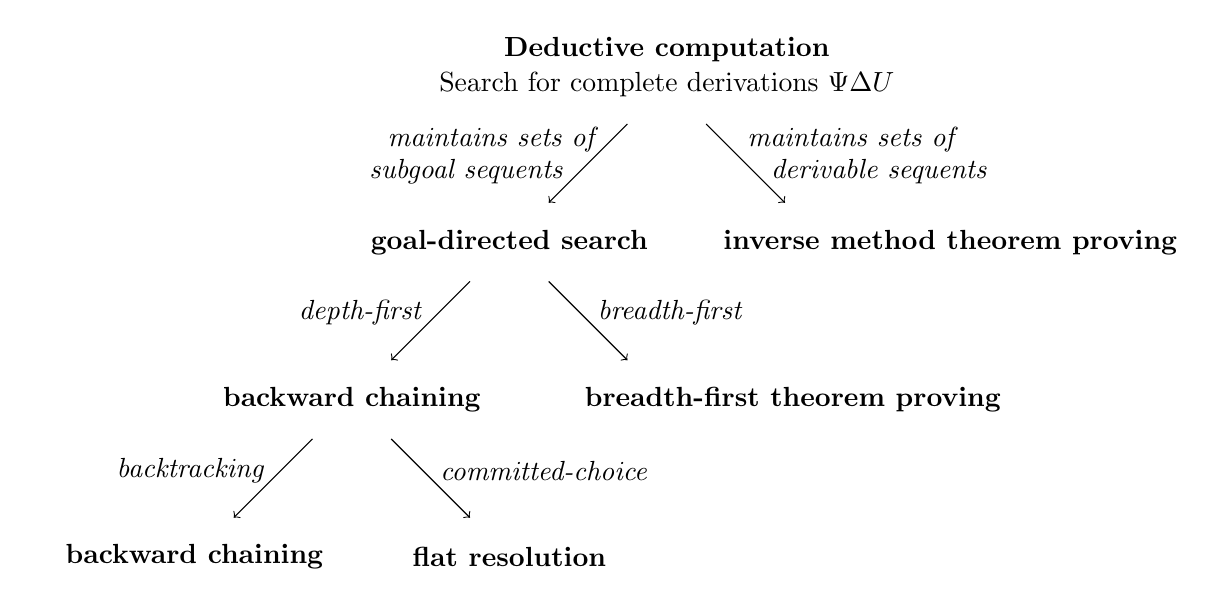
\begin{tikzpicture}
\draw (0,10) node{~};
\draw (8,10.45) node{\bf Deductive computation};
\draw (8,10) node{Search for complete derivations $\foc{\Psi}{\Delta}{U}$};
\draw [->] (7.5,9.5) -- (6.5,8.5); 
\draw (7.2,9.3) node[left]{\it maintains sets of};
\draw (6.8,8.9) node[left]{\it subgoal sequents};
\draw [->] (8.5,9.5) -- (9.5,8.5); 
\draw (8.9,9.3) node[right]{\it maintains sets of};
\draw (9.2,8.9) node[right]{\it derivable sequents};
%
\draw (6,8) node{\bf goal-directed search};
\draw [->] (5.5,7.5) -- (4.5,6.5); 
\draw (5,7.1) node[left]{\it depth-first};
\draw [->] (6.5,7.5) -- (7.5,6.5); 
\draw (7,7.1) node[right]{\it breadth-first};
%
\draw (4,6) node{\bf backward chaining};
\draw [->] (3.5,5.5) -- (2.5,4.5); 
\draw (3,5.1) node[left]{\it backtracking};
\draw [->] (4.5,5.5) -- (5.5,4.5); 
\draw (5,5.1) node[right]{\it committed-choice};
%
\draw (2,4) node{\bf backward chaining};
%
\draw (6,4) node{\bf flat resolution};
%
\draw (9.6,6) node{\bf breadth-first theorem proving};
%
\draw (11.6,8) node{\bf inverse method theorem proving};
%
% \draw (13,10.45) node{\bf Trace computation};
% \draw (13,10) node{Search for partial proofs 
%    $(\Psi; \Delta) \leadsto^* (\Psi'; \Delta')$};
% \draw [->] (12.5,9.5) -- (11.5,8.5); 
% \draw [->] (13.5,9.5) -- (14.5,8.5); 
%
\end{tikzpicture}
\caption{A rough taxonomy of deductive computation}
\label{fig:computation-taxonomy}
\end{figure}

Figure~\ref{fig:computation-taxonomy} gives an taxonomy (incomplete
and imperfect) of the forms of deductive computation mentioned in this
section. Note that, while we will generally use {\it backward
  chaining} to describe backtracking search, backward chaining does
not always imply full backtracking and partial completeness. This
illustration, and the preceding discussion, leaves out many important
categories, especially tabled logic programming, and many potentially
relevant implementation choices, such as breath-first versus
depth-first or parallel exploration of the success continuation.


\subsection{Concurrent computation}
\label{sec:framework-logicprog-trace}


Concurrent computation is the search for {\it partial} proofs of
sequents. As the name suggests, in \sls~concurrent computation is
associated with the search for partial proofs of the judgment
$\islax{A^+}$, which correspond to traces $(\Psi;
\Delta) \leadsto^* (\Psi'; \Delta')$. 

The paradigm we will primarily associate with concurrent computation
is {\it forward chaining}, which implies that we take an initial
process state $(\Psi;\Delta)$ and allow it to evolve freely by the
application of synthetic transitions. Additional conditions can be
imposed on forward chaining: for instance, synthetic transitions like
$(\Delta, x{:}\ispers{\susp{p^+_\mpers}}) \leadsto (\Delta,
x{:}\ispers{\susp{p^+_\mpers}}, y{:}\ispers{\susp{p^+_\mpers}})$ that
do not meaningfully change the state can be excluded (if a persistent
proposition already exists, two copies of that proposition don't add
anything).\footnote{Incidentally, Lollimon implements this restriction
  and Celf does not.} Forward chaining with this restriction in a
purely-persistent logic is strongly associated with the Datalog
language and its implementations; we will refer to forward chaining in
persistent logics as {\it saturating logic programming} in Chapter
8. Forward chaining does not always deal with partially-unspecified
terms; when persistent logic programming languages support forward
chaining with partially-unspecified terms variables, it is called {\it
  hyperresolution} \cite{fermuller01resolution}.

The presence of ephemeral or ordered resources in substructural logic
means that a process state may evolve in multiple
mutually-incompatible ways. {\it Committed choice} is a version of
forward chaining that never goes back and reconsiders alternate
evolutions from the initial state. Just as the default interpretation
of backward chaining includes backtracking, we will consider the
default interpretation of forward chaining to be committed choice,
following \cite{lopez05monadic}.  An
alternate interpretation of forward chaining would consider multiple
evolutionary paths, which is a version of {\it model checking}.  The
model checking problem takes an initial process state $(\Psi;\Delta)$
or a set of initial states and attempts to enumerate or otherwise
characterize the entire set of states $(\Psi'; \Delta')$ such that
$(\Psi; \Delta) \leadsto^* (\Psi'; \Delta')$. Trace computation that
works backwards from a final state instead of forward from an initial
state can also be considered, and {\it planning} can be seen as
specifying both the initial and final process states and trying to
extrapolate a trace between them by working in both directions.

Outside of this work and Saurin's work on Ludics programming
\cite{saurin08towards}, there is not much work on explicitly
characterizing and searching for partial proofs in substructural
logics.\footnote{As such, ``concurrent computation,'' while
  appropriate for \sls, may or may not prove to be a good name for the
  general paradigm.}  Other forms of computation can be characterized
as trace computation, however.  Multiset rewriting and languages like
GAMMA can be partially or completely understood in terms of forward
chaining in linear logic \cite{cervesato09relating,paola96linear}, and
the ordered aspects of \sls~allow it to capture fragments of rewriting
logic. Multiset rewriting and rewriting logic both have
implementations that correspond to the committed choice interpretation
and to the model checking interpretations.  


% not consider unspecified variables and is largely free of the resource
% management problems that appear in backward-chaining deductive
% computation for substructural logics. In previous work, we designed a
% forward chaining interpreter for linear logic that admits abstract
% reasoning about the asymptotic complexity of logical specifications
% \cite{simmons08linear}, but this is outside the scope of this thesis.



\subsection{Integrating deductive and trace computation}

In the logic programming interpretation of CLF used by Lollimon and
Celf, backtracking backward chaining is associated with the deductive
fragment, and committed-choice forward chaining is associated with the
lax modality. We will refer to an adaptation of the Lollimon/Celf
semantics to \sls~as LCI (``Lollimon/Celf Interpreter'') for
brevity in this section.

Forward chaining and backward chaining have an uneasy relationship in
LCI. To see why, consider the following \sls~signature:
\begin{align*}
 \Sigma_{\it Demo} = \cdot, 
~&{\sf posA} : {\sf prop}\,{\sf ord}, 
~~{\sf posB} : {\sf prop}\,{\sf ord}, 
~~{\sf posC} : {\sf prop}\,{\sf ord}, 
~~{\sf negD} : {\sf prop},\\
~&{\sf fwdruleAB} : {\sf posA} \lefti {\ocircle}{\sf posB},\\
~&{\sf fwdruleAC} : {\sf posA} \lefti {\ocircle}{\sf posC},\\
~&{\sf bwdrule} : ({\sf posA} \lefti {\ocircle}{\sf posB}) \lefti {\sf negD}
\end{align*}

In an empty context, there is only one derivation of ${\sf negD}$
under this signature: it is represented by the proof term ${\sf
  bwdrule}\,(\lambda x.\,\tlet{\trstep{y}{{\sf
      fwdruleAB}\,x}}{y})$. The partially complete interpretation of
backward chaining stipulates that an interpreter tasked with finding a
proof of ${\sf negD}$ should either find this proof or never
terminate, but LCI only admits this interpretation for purely
deductive-proofs. To see why, consider backward-chaining search
attempting to prove ${\sf negD}$ in a closed context.  This can only
be done with the rule ${\sf bwdrule}$, generating the subgoal ${\sf
  posA} \lefti {\ocircle}{\sf posB}$.  At this point, LCI will switch
from backward chaining to forward chaining and attempt to satisfy this
subgoal by constructing a trace $(x{:}\istrue{\susp{\sf posA}})
\leadsto (y{:}\istrue{\susp{\sf posB}})$.

There are {\it two} nontrivial traces in this signature starting from
the process state $(x{:}\istrue{\susp{\sf posA}})$ -- the first is
$(\trstep{y}{{\sf fwdruleAB}\,x}) :: (x{:}\istrue{\susp{\sf posA}})
\leadsto (y{:}\istrue{\susp{\sf posB}})$, and the second is
$(\trstep{y}{{\sf fwdruleAC}\,x})::(x{:}\istrue{\susp{\sf posA}})
\leadsto (y{:}\istrue{\susp{\sf posC}})$.  Forward chaining can
plausibly come up with either one, and if it happens to derive the
second one, the subgoal fails. LCI then tries to backtrack to find
other rules that can prove the conclusion ${\sf negD}$, but there are
none, so LCI will report that it failed to prove ${\sf negD}$.

This example indicates that it is difficult to make backward chaining
(in its default backtracking form) reliant on committed-choice forward
chaining (in its default committed-choice form) in the style of
Lollimon or Celf. Either we can restrict forward chaining to confluent
systems (excluding $\Sigma_{\it Demo}$) or else we can give up on the
usual partially complete interpretation of backward chaining.  In the
other direction, however, it is entirely natural to make forward
chaining dependent upon backward chaining. The fragment of CLF that
encodes this kind of computation was labeled the {\it semantic
  effects} fragment by DeYoung \cite{deyoung09reasoning}. At the
logical level, the semantic effects fragment of \sls~removes the right
rule for ${\ocircle}A^+$, which corresponds to the proof term
$\tlet{T}{V}$.  As discussed in
Section~\ref{sec:framework-concurrent}, let-expressions are the only point
where traces are included into the language of
deductive terms.

\section{Design decisions}
\label{sec:designdecisions}

Aside from ordered propositions, there are several significant
differences between the framework \sls~presented in this chapter and
the existing logical framework CLF, including the presence of positive
atomic propositions, the introduction of traces as an explicit
notation for partial proofs, the restriction of the term language to
LF, and the presence of equality $\lf{t} \doteq \lf{s}$ as a
proposition. In this section, we will discuss design choices that were
made in terms of each of these features, their effects, and what
choices could have been made differently.

\subsection{Pseudo-positive atoms}
\label{sec:pseudopositive}

Unlike \sls, the CLF framework does not include positive
atomic propositions. Positive atomic propositions make it easy to
characterize the synthetic transitions associated with a particular
rule. For example, if ${\sf foo}$, ${\sf bar}$, and ${\sf baz}$ are
all linear atomic propositions, then the presence of a rule $\left({\sf foo}
\fuse {\sf bar} \lefti {\ocircle}{\sf baz}\right)$ in the signature is associated
with synthetic transitions of the form
%
$(\Psi; \matchconj{\Delta}{\matchconj{x{:}\iseph{\susp{\sf
        foo}}}{y{:}\iseph{\susp{\sf bar}}}})
 \leadsto
 (\Psi; \mkconj{\Delta}{z{:}\iseph{\susp{\sf baz}}})$.
%
The presence of the
rule $\sf r$ enables steps of this form, and every step made by
focusing on the rule has this form.

CLF has no positive propositions, so the closest analogue that we can
consider is where ${\sf foo}$, ${\sf bar}$, and ${\sf baz}$ are
negative propositions, and the rule ${\gnab}{\sf foo} \fuse
{\gnab}{\sf bar} \lefti \ocircle({\gnab}{\sf baz})$ appears in the
signature. Such a rule is associated with synthetic transitions of the
form
%
$(\Psi; \matchconj{\Delta}{\matchconj{\Delta_1}{\Delta_2}}) \leadsto
(\Psi; \mkconj{\Delta}{z{:}\istrue{{\sf baz}}})$ such that
$\foc{\Psi}{\restrictto{\Delta_1}{\meph}}{\istrue{\susp{\sf foo}}}$
and $\foc{\Psi}{\restrictto{\Delta_2}{\meph}}{\istrue{\susp{\sf
      bar}}}$. In \sls, it is a relatively simple syntactic criterion
to enforce that a sequent like $\foc{\Psi}{\Delta_1}{\istrue{\susp{\sf
      foo}}}$ can only be derived if $\Delta_1$ matches
$x{:}\sf{foo}$; we must simply ensure that there are no propositions
of the form $\ldots \lefti {\sf foo}$ or $\ldots \righti {\sf foo}$ in
the signature or context. (In fact, this is essentially the
\sls~version of the subordination criteria that allows us to conclude
that an LF type was only inhabited by variables
Section~\ref{sec:slsframework}.)  Note that, in full \ollll, this task
would not be so easy: we might prove $\istrue{\susp{\sf foo}}$
indirectly by forward chaining. This is one reason why association of
traces with the lax modality is so important!

When it is the case that  $\foc{\Psi}{\Delta_1}{\istrue{\susp{\sf
      foo}}}$ can only be derived if $\Delta_1$ matches
$x{:}\sf{foo}$, we can
associate the rule ${\gnab}{\sf foo} \fuse
{\gnab}{\sf bar} \lefti \ocircle({\downarrow}({\gnab}{\sf baz}))$
with the synthetic transition $(\Psi;
\matchconj{\Delta}{\matchconj{x{:}{\islvl{\sf foo}}}{y{:}{\islvl{\sf
        bar}'}}}) \leadsto (\Psi; \mkconj{\Delta}{z{:}\iseph{\susp{\sf
      baz}}})$ under the condition that neither $\mlvl$ or $\mlvl'$
are $\mtrue$.
Negative atomic propositions that can only be concluded when they are
the sole member of the context, like ${\sf foo}$ and ${\sf bar}$ in
this example, can be called {\it
  pseudo-positive}. Pseudo-positive atoms can actually be used a bit
more generally than \sls's positive atomic propositions. A positive
atomic proposition is necessarily associated with one of the three
judgments $\mtrue$, $\meph$, or $\mpers$, but pseudo-positive
propositions can associate with any of the contexts. This,
incidentally, gives pseudo-positive atoms in CLF or \sls~the flavor of
positive atomic propositions under Andreoli's atom optimization
(Section~\ref{sec:atomopt}).

It is, of course, possible to consistently associate particular
pseudo-positive propositions with particular modalities, which means
that pseudo-positive propositions can subsume the positive
propositions of \sls. The tradeoff between positive and
pseudo-positive propositions could be resolved either way. By
including positive atomic propositions, we made \sls~more complicated,
but in a local way -- we needed a few more kinds and a few more
rules. On the other hand, if we used pseudo-positive propositions, the
notion of synthetic transitions would be intertwined with the
subordination-like analysis that enforces their correct usage.

\subsection{The need for traces}
\label{sec:whytraces}

One of the most important differences between \sls~and its
predecessors, especially CLF, is that traces are treated as
first-class syntactic objects. This allows us to talk about 
partial proofs and thereby encode our earlier 
money-store-battery-robot example as a trace with this type:
\begin{align*}
& \left(
 x{:}\iseph{\susp{\sf 6bucks}}, ~~
 f{:}\iseph{({\sf battery} \lefti {\ocircle}{\sf robot})}, ~~
 g{:}\ispers{({\sf 6bucks} \lefti {\ocircle}{\sf battery})}
\right)
\\
\leadsto^* &
\left(
 z{:}\iseph{\susp{\sf robot}}, ~~
 g{:}\ispers{({\sf 6bucks} \lefti {\ocircle}{\sf battery})}
\right)
\end{align*}
It is also possible to translate the example from Chapter~2
as a {\it complete} proof of the following proposition:
\[
  {\sf 6bucks} 
      \fuse {\gnab}({\sf battery} \lefti {\ocircle}{\sf robot})
      \fuse {!}({\sf 6bucks} \lefti {\ocircle}{\sf battery})
     \lefti
     {\ocircle}{\sf robot}
\]

Generally speaking, we can try to represent a trace $T :: (\Psi;
\Delta) \leadsto^* (\Psi'; \Delta')$ as a closed deductive proof
$\lambda P.\,\tlet{T}{V}$ of the proposition $(\exists
\Psi.\,{\fuse}\Delta) \lefti {\ocircle}(\exists
\Psi'.\,{\fuse}\Delta)$,\footnote{The notation ${\fuse}{\Delta}$ fuses
  together all the propositions in the context. For example, if
  $\Delta = w{:}\iseph{\susp{p^+_\meph}} \fuse x{:}\istrue{A^-},
  y{:}\iseph{B^-}, z{:}\ispers{C^-}$, then ${\fuse}{\Delta} = p^+_\meph
  \fuse {\downarrow}A^- \fuse {\gnab}B^- \fuse {!}C^-$. The notation
  $\exists \Psi. A^+$ turns all the bindings in the context $\Psi =
  \lf{a_1}{:}\tau_1,\ldots,\lf{a_n}{:}\tau_n$ into existential
  bindings $\exists \lf{a_1}{:}\tau_1\ldots\exists
  \lf{a_n}{:}\tau_n.A^+$.}  where the pattern $P$ re-creates the initial
process state $(\Psi; \Delta)$ and the all the components of the final
state are captured in the value $V$.  The problem with this approach
is that the final proposition is under no particular obligation to
faithfully
capture the structure of the final process state. This can be seen in
the example above: to actually capture the structure of the final
process state, we should have concluded ${\sf robot} \fuse {!}({\sf
  6bucks} \lefti {\ocircle}{\sf battery})$ instead of simply ${\sf
  robot}$. It is also possible to conclude any of the following:
\smallskip
\begin{enumerate}
\item ${\sf robot} \fuse {!}({\sf 6bucks} \lefti {\ocircle}{\sf
  battery}) \fuse {!}({\sf 6bucks} \lefti {\ocircle}{\sf
  battery})$, or 
\item ${\sf robot} \fuse {\downarrow}({\sf 6bucks} \lefti {\ocircle}{\sf
  battery}) \fuse {\gnab}({\sf 6bucks} \lefti {\ocircle}{\sf
  battery})$, or even
\item ${\sf robot}  \fuse {\gnab}({\sf 6bucks} \fuse {!}({\sf battery} \lefti {\ocircle}{\sf robot} \}) \lefti {\ocircle}{\sf robot})
  \fuse {\downarrow}({\sf robot}
\lefti {\ocircle}{\sf robot})$.
\end{enumerate}
\smallskip 
%
The problem with encoding traces as complete proofs, then, is that
values cannot be forced to 
precisely capture the structure of contexts, especially when there are
no variables or persistent propositions. Cervesato and Scedrov
approach this problem by severely restricting the logic and changing
the interpretation of the existential quantifier so that it acts like
a nominal quantifier on the right \cite{cervesato09relating}. The
introduction of traces allows us to avoid similar restrictions in
\sls.

Despite traces being proper syntactic objects, they are not
first-class concepts in the theory: they are derived from focused
\ollll~terms and interpreted as partial proofs. Because hereditary
substitution, identity expansion, and focalization are only defined on
complete \ollll~proofs, these theorems and operations only apply by
analogy to the deductive fragment of \sls; they do not apply to
traces.  In joint work with Deng and Cervesato, we considered a
presentation of logic that treats process states and traces as
first-class concepts and reformulates the usual properties of cut and
identity in terms of coinductive simulation relations on process
states \cite{deng12relating}. We hope that this work will eventually
lead to a better understanding of traces, but the gap remains quite
large.

% In \cite{deng12relating}, we presented the {\it logical preorder} as a
% relation $\Delta_1 \preceq \Delta_2$ between propositional process states
% that holds whenever, for all $\Theta$ and $U$, we have that
% $\tackon{\Theta}{\Delta_1} \vdash U$ implies $\tackon{\Theta}{\Delta_2}
% \vdash U$. An elegant property, {\it harmony}, relates the logical 
% preorder to cut admissibility and identity expansion. 


% \subsection{A logic of traces}

% Traces in \sls~are syntactic objects. They are not, however,
% first-class objects in the theory: they are derived from focused
% \ollll~terms and explained as partial proofs. Because hereditary
% substitution, identity expansion, and focalization are only defined on
% complete \ollll~proofs, these theorems and operations only apply by
% analogy to the deductive fragment \sls; they do not apply to traces.

% In \cite{deng12relating}, we presented the {\it logical preorder} as a
% relation $\Delta_1 \preceq \Delta_2$ between propositional process states
% that holds whenever, for all $\Theta$ and $U$, we have that
% $\tackon{\Theta}{\Delta_1} \vdash U$ implies $\tackon{\Theta}{\Delta_2}
% \vdash U$. An elegant property, {\it harmony}, relates the logical 
% preorder to cut admissibility and identity expansion. 

\subsection{LF as a term language}
\label{sec:why-not-fully-dependent}

The decision to use LF as a first-order domain of quantification
rather than using a fully-dependent system is based on several
considerations. First and foremost, this choice was sufficient for the
purposes of this thesis. In fact, for the purposes of this thesis, we
could have used an even simpler term language of simply-typed LF
\cite{pfenning08church}. Two other logic programming interpretations
of \sls-like frameworks, Lollimon \cite{lopez05monadic} and Ollibot
\cite{pfenning09substructural}, are in fact based on simply-typed term
languages. Canonical LF and Spine Form LF are, at this point,
well-understood enough that the additional overhead of fully
dependently-typed terms is not a significant burden, and there are
many examples beyond the scope of this thesis where dependent types are
useful.

On a theoretical level, it is a significant simplification when we
restrict ourselves to {\it any} typed term language with a reasonable
notion of equality and simultaneous substitution. The conceptual
priority in this chapter is clear: Section~\ref{sec:sls-termlanguage}
describes object terms, Section~\ref{sec:slsframework} describes proof
terms as a fragment of focused \ollll, and
Section~\ref{sec:framework-concurrenteq} describes a coarser
equivalence on proof terms, concurrent equality. If the domain of
first-order of quantification was \sls~terms, these three
considerations would be mutually dependent -- we would need to
characterize concurrent equality before presenting the logic
itself. For the purposes of showing that a logical framework can be
carved out from a focused logic -- the central thesis of this and the
previous two chapters -- it is easiest to break this circular
dependency. We conjecture that this complication is no great obstacle,
but this thesis avoids the issue.

On a practical level, there are advantages to using a well-understood
term language. The \sls~prototype implementation
(Section~\ref{sec:prototype}) uses the mature type reconstruction
engine of Twelf to reconstruct LF terms. Schack-Nielsen's
implementation of type reconstruction for Celf is complicated by the
requirements of dealing with type reconstruction for a substructural
term language, a consideration that is orthogonal to this
thesis \cite{schacknielsen08celf}. 

Finally, it is not clear that the addition of full CLF-like dependency
comes with great expressive benefit. 
% Even in LF and Twelf, many
% interesting specifications could be encoded in a two-level version of
% the language: a simply-typed object term language and a
% dependently-typed proof term language with first-order quantification
% over object terms. This restriction is sufficient for settings such as
% Harper's comprehensive survey of programming language design
% \cite{harper12practical},\footnote{Harper's metatheory also extends LF
%   by drawing a distinction between standard variables and nominal
%   parameters, but this is an orthogonal point.} and it is built in to
% the educational proof assistant SASyLF \cite{aldrich08sasylf}. 
In LF and Twelf, the ability to use full dependent types is critical
in part because it allows us to express {\it metatheorems} -- theorems
about the programming languages and logics we have encoded, like
progress and preservation for a programming language or cut
admissibility for a logic. Substructural logical frameworks like LLF
and CLF, in contrast, have not been successful in capturing
metatheorems with dependent types. Instead, metatheorems have been
done in persistent frameworks. Crary proved theorems about linear
logics and languages in LF using the technique of explicit contexts
\cite{crary10higher}. Reed was able to prove cut admissibility for
linear logic and preservation for the LLF encoding of Mini-ML in HLF,
a persistent extension to LF that uses an equational theory to capture
the structure of substructural contexts \cite{reed09hybrid}.

% But in substructural logical frameworks like Linear LF, full
% dependency has been found to be {\it insufficient} for expressing
% metatheorems, which motivated the development of Hybrid LF as a
% framework for writing metatheorems about LF \cite{reed09hybrid}. The
% implementation of Hybrid LF effectively creates a stratification like
% \sls's -- full LF as an object term language, a linear logical
% framework with first-order quantification over object language terms,
% and a hybrid language that can inspect both LF object terms and linear
% proof terms.



\subsection{Variations on concurrent equality}

Concurrent equality is related to the equivalence relation induced by
{\it multifocusing} \cite{chaudhuri08canonical}. Multifocusing has
only been explored carefully in the context of classical linear
logic. We conjecture that a suitably-defined notion of multifocusing
for \ollll~would be in bijective correspondence with \sls~terms modulo
concurrent equivalence, at least if we omit unification. Of course,
without a formal notion of multifocusing for intuitionistic logic, this
conjecture is impossible to state explicitly.

The interactions between unification and concurrent equality are
delicate, and we do not claim that the answers we give here are
final. In Section~\ref{sec:independency}, we motivated both the
independency requirement that $\emptyset = {\bullet}S_1 \cap
{\ast}S_2$ and the requirement that $\emptyset = {\ast}S_1 \cap
{\bullet}S_2$ by giving ill-typed counterexamples. The violation of
either condition does not, in general, imply that $S_2; S_1$ will be
ill-typed, however. This indicates that it might be possible to give a
more precise condition that admits a coarser notion of concurrent
equality.

% For both
% conditions, however, there are steps $S_1$ and $S_2$ where the
% $S_1; S_2$ and $S_2; S_1$ are both well-tyled traces even though
% one of these independency requirements is not satisfied.


% coincide with the equivalence  \sls~

% ${a^+} \supset (a^+ \supset {\uparrow}b^+) \supset 
%   ({\downarrow}{\uparrow}b^+ \supset c^-) \supset c^-$. 

% It is not obvious that our treatment of the interaction between 
% unification and concurrent equivalence is the right one. 

% \subsection{Concurrent equality and multifocusing}

% Concurrent equality is related to the equivalence relation induced by
% {\it multifocusing} \cite{chaudhuri08canonical}. Multifocusing is a
% concept, 

% One reason multifocusing is 

%  that has only been carefully explored in classical linear
% logic; the central change is that the rules which begins a focusing
% phase (in our presentation of MELL there were three: ${\it focus_L}$,
% ${\it focus_R}$, and ${\it copy}$) are allowed to simultaneously pull
% other propositions into focus.  As an illustration, if we reuse our
% notation from Section~\ref{sec:linnote} we can present the following
% plausible candidates for the multifocus rules in an intuitionistic
% system:
% \[
% \infer[{\it focus}_L]
% {\mildseq{\Gamma}{\Delta / A_1^-, \ldots, A_n^- }{U}}
% {n > 1
%  &
%  \mildseq{\Gamma}{\Delta, [A_1^-], \ldots, [A_n^-]}{U}}
% \quad
% \infer[{\it focus}_R]
% {\mildseq{\Gamma}{\Delta / A_1^-, \ldots, A_n^-}{C^+}}
% {n \geq 1
%  &
%  \mildseq{\Gamma}{\Delta, [A_1^-], \ldots, [A_n^-]}{[C^+]}}
% \]
% Multifocusing, however,
% appears to provide an even coarser notion of equivalence on focused
% proofs than concurrent equality does. In particular, the two
% distinct focusing proofs below are not concurrently equal: the proof
% on the right succeeds at proving $\langle c^- \rangle$ in one step,
% but leaves a subgoal in which $b^+$ is proved indirectly, whereas the
% proof at the right first transitions from having $\langle a^+ \rangle$
% and $a^+ \lolli {\uparrow} b^+$ resources to having a $\langle b^+
% \rangle$ resource, and only then proves $\langle c^- \rangle$, leaving
% a subgoal in which $b^+$ is proved directly.
% \[
% \infer
% {\mildseq{\cdot}
%   {~~
%    \langle a^+ \rangle, ~
%    a^+ \lolli {\uparrow}b^+, ~
%    {\downarrow}{\uparrow}b^+ \lolli c^-
%    ~~}
%   {~~\langle c^- \rangle}}
% {\infer
% {\mildseq{\cdot}
%   {~~
%    \langle a^+ \rangle, ~
%    a^+ \lolli {\uparrow}b^+
%    ~~}
%   {b^+}}
% {\infer
% {\mildseq{\cdot}
%   {~~
%    \langle b^+ \rangle
%    ~~}
%   {b^+}}
% {}}}
% \deduce{\mathstrut}
% {\deduce{\mathstrut}
% {\mbox{\it vs.}\mathstrut}}
% \infer
% {\mildseq{\cdot}
%   {~~
%    \langle a^+ \rangle, ~
%    a^+ \lolli {\uparrow}b^+, ~
%    {\downarrow}{\uparrow}b^+ \lolli c^-
%    ~~}
%   {~~\langle c^- \rangle}}
% {\infer
% {\mildseq{\cdot}
%   {~~
%    \langle b^+ \rangle, ~
%    {\downarrow}{\uparrow}b^+ \lolli c^-
%    ~~}
%   {~~\langle c^- \rangle}}
% {\infer
% {\mildseq{\cdot}
%   {~~
%    \langle b^+ \rangle
%    ~~}
%   {~~b^+}}
% {}}}
% \]
% Despite the lack of a full account of intuitionistic multifocusing, we
% can observe that the analogue of this sequent in classical linear
% logic has only one multifocused proof, and it is reasonable to
% conjecture that an account of multifocusing for intuitionistic logic
% would also relate these proofs. In classical linear logic,
% multifocusing offers a very fundamental normal form: any two proofs
% that can be made equal by locally permuting inference rules have the
% same multifocused proof.

% CLF's restricted form of concurrent equality will be sufficient for
% the logical framework in Chapter 4. In fact, for the fragment of the
% the logic in Chapter 3 that comprises our logical framework in Chapter
% 4, I conjecture that concurrent equality and the equality given by
% multifocusing coincide.\footnote{This obviously means that the example
%   above will be outside the logical fragment that comprises the logical
%   framework.}  This conjecture is obviously difficult to make precise,
% much less prove, without a general theory of multifocusing in
% intuitionistic logic.


% \subsection{A warning about normalization}
% \label{sec:warning}

% In our earlier discussion of hereditary substitution and canonical
% forms in Section~\ref{sec:linlogicalframeworks}, we mentioned that the
% normalization theorem provided by hereditary substitution was weaker
% than the so-called weak normalization theorem for LF. That is because
% the weak normalization theorem says that any well-typed term can be
% converted into a canonical ($\beta$-normal and $\eta$-long) term by a
% particular series of $\beta$ and $\eta$ conversions. It is
% self-evident, by this statement of the theorem, that the resulting
% canonical term is equivalent to the original term.

% On the other hand, when we use hereditary substitution in the obvious
% way to obtain a Canonical LF term from an arbitrary non-canonical LF
% term, we gain {\it no guarantees} about the relationship between the
% non-canonical LF term and the Canonical LF term. The statement of the
% theorem does not preclude taking a $\beta$-normal, $\eta$-long LF term
% (like $\lambda x. \lambda y. x$ of type $p \rightarrow p \rightarrow
% p$ for some atomic type $p$) into a structurally different Canonical
% LF term (like $\lambda x. \lambda y. y$, which also has type $p
% \rightarrow p \rightarrow p$). It is possible to gain such a guarantee
% for LF, as Martens and Crary have shown in unpublished work
% \cite{martens11mechanizing}, but this result is a non-trivial statement
% about the constructive content of the normalization theorem. 

% In our setting, we should be concerned that we might take a focused
% proof, turn it into an unfocused proof by the obvious de-focalization
% procedure (the constructive content of
% Theorem~\ref{thm:linfocsound}), and then turn it back into a focused
% proof by focalization (the constructive content of
% Theorem~\ref{thm:linfoccomplete}) only to obtain a proof that was not
% identical or even related. This is not at all a merely hypothetical
% concern. We can run the mechanized structural focalization result from
% \cite{simmons11structural} on a persistent proposition,
% %
%    $a^+ \supset 
%    {\downarrow}(a^+ \supset {\uparrow}b^+) \supset
%    {\downarrow}({\downarrow}{\uparrow}b^+ \supset c^-) \supset
%    c^-$, 
% %
% which is similar to the example from
% Section~\ref{sec:linconcurrenteq}.  In persistent logic (as in
% linear logic) that proposition has two focused propositions that
% are probably multifocusing equivalent (given a reasonable intuitionistic
% notion of multifocusing) but that are not concurrently equivalent
% under the proposed definition of concurrent equality. 
% However, if we take the focused proof that focuses 
% first on $a^+ \supset {\uparrow}b^+$, transform it into an unfocused 
% proof, and then re-focus it, we will get the proof that focuses 
% first on ${\downarrow}{\uparrow}b^+ \supset c^-$. Focalization,
% in other words, is not a partial inverse of de-focalization in the structural
% focalization development, except maybe modulo the (as yet undefined)
% equivalence relation established by multifocusing. 

% This example illustrates why we must be careful, but it is not a fatal
% flaw for two reasons. The first reason is the aforementioned
% conjecture that, for the restricted logical fragment defined in
% Chapter 4 as the basis of our logical framework, the focalizations of
% two proofs are concurrently equal if and only if the original proofs
% are convertible by local permutations of rules, the same condition
% that multifocusing satisfies. If this conjecture holds, it ought to be
% the case that, modulo this coarser equivalence, focalization {\it is}
% a partial inverse of de-focalization. Second, what is really at stake
% here is our ability to write down non-normal proofs in a logical
% framework that then normalizes them -- which is what the Twelf
% implementation of LF and the Celf implementation of CLF do -- with the
% confidence that we can look at a non-normal proof and know its
% corresponding canonical form. In this thesis, we will be content to
% work throughout with focused proofs and their analogues, so we can
% afford to leave questions about convertability and weak normalization
% to future work.

